% Author-review manuscript. Evidence boundary and source map: README.md and WRITING_NOTES.md.
% Historical Validation tables are traced to audited selected-run records; see the evidence map.
\documentclass[runningheads]{llncs}
\usepackage[T1]{fontenc}
\usepackage{amsmath}
\usepackage{newtxtext}
\usepackage[varvw]{newtxmath}
\usepackage{booktabs,array}
\usepackage{algorithm}
\usepackage{algpseudocode}
\usepackage{graphicx}
\usepackage{tikz}
\usetikzlibrary{arrows.meta,positioning,fit,calc}
\usepackage[hidelinks]{hyperref}
\providecommand{\Description}[1]{}
\newcommand{\method}{TitanTPP}
\newcommand{\GELU}{\operatorname{GELU}}
\newcommand{\softplus}{\operatorname{softplus}}
\newcommand{\Nrm}{\operatorname{norm}}
\newcommand{\Hcal}{\mathcal{H}}
\newcommand{\pmval}[2]{\ensuremath{#1\,{\scriptstyle\pm}\,#2}}
\definecolor{enc}{RGB}{226,237,248}
\definecolor{hist}{RGB}{218,239,231}
\definecolor{head}{RGB}{249,237,212}
\definecolor{ink}{RGB}{44,63,78}

\begin{document}
\title{TitanTPP: Local and Recurrent History Correction\texorpdfstring{\\}{ }for Event Quantity Prediction}
\titlerunning{TitanTPP: History Correction for Event Quantity Prediction}
\author{Anonymous Authors}
\authorrunning{Anonymous Authors}
\institute{Affiliations withheld for anonymous review}
\maketitle

\begin{abstract}
Event forecasting requires predicting how much will occur as well as when it will occur. A history encoder supplies information for both predictions, but this does not establish whether a separate path through recent observed states is useful. We study this question in TitanTPP, a causal attention model with an explicit correction path. The representative architecture applies a three-position correction to queries, keys, and values, then adds a gated recurrent residual between attention blocks. A separate comparison examines prototype retrieval with time and quantity queries. In a completed 54-run study of an earlier MLP8 correction, adding the correction reduced validation quantity RMSE in all 18 paired comparisons across three datasets. The benefit was largest on Taxi, where mean RMSE fell by 13.0--14.1\%, but recorded-time likelihood deteriorated. Prototype addition was less consistent. These findings motivate controls that separate previous-state input from additional parameters, and split-query retrieval from general query learning. The CNN+GRU controls remain under evaluation. We report an earlier common-head comparison, the completed MLP8 ablation, and one supplementary Instacart fit as development-validation evidence.
\keywords{Event forecasting \and Quantity prediction \and History correction \and Temporal point processes}
\end{abstract}

\section{Introduction}
Intermittent demand alternates between periods without demand and nonzero observations whose sizes can vary. Forecasting therefore requires an account of both the interval to the next demand and its quantity. Croston's method separates demand size from the interval between nonzero observations~\cite{croston1972forecasting}; later renewal models place this event-based description within a probabilistic framework~\cite{turkmen2021renewal}.

Temporal point processes provide a natural representation of event arrivals. Several neural formulations, including RMTPP and Transformer Hawkes Process, predict categorical event types alongside their occurrence times~\cite{du2016rmtpp,zuo2020thp}. Demand quantity has a numerical magnitude, however, and a type-classification objective does not directly account for the size of a quantity error. The distinction concerns categorical types versus numerical values, rather than discrete versus continuous data: demand counts can themselves be integer-valued. Point processes are not restricted to categorical marks. Deep renewal models already address demand size and arrival intervals, while mixed-attribute event models support numerical attributes~\cite{turkmen2021renewal,draxler2025flextpp}.

Our question concerns the representation of observed history within this numerical prediction task. Recurrence, attention, and continuous-time states already summarize earlier events~\cite{mei2017nhp,yang2022anhp,chang2025s2p2}. Yet this does not determine whether a separate path through recent observed states improves quantity prediction. We ask whether an explicit correction adds useful structure beyond a history-aware encoder and a control with the same active parameter budget. All arms receive numerical event inputs and share quantity and timing output heads, so their comparison concerns the correction and retrieval paths.

We investigate this question with \method. The representative CNN+GRU54 model combines two forms of correction. A local path adjusts attention queries, keys, and values using the current and two preceding observed positions. A recurrent path adds a projected GRU state between the two attention blocks. The suffix 54 denotes the GRU state width. Both paths are residual, allowing the initial model to retain the shared encoder computation. They provide a particular way to reuse history, rather than supplying information unavailable to the causal encoder.

An earlier MLP8 version gives a reason to examine the correction more closely. Across Taxi, Intermittent, and RAF Spare Parts, switching on its explicit previous-state path improved overall quantity RMSE in all 18 comparisons formed by three seeds and two prototype settings. Yet the strongest quantity gains came with worse timing likelihood on Taxi. Moreover, adding prototypes to the corrected model did not improve quantity RMSE consistently across datasets. This pattern motivates two separate questions: the value of an explicit history path, and the value of the rule used to retrieve from a learned prototype bank.

The distinction matters for attribution. Removing the history path also removes parameters, so that comparison alone cannot identify the benefit of its input. We therefore include a control with the same number of active correction parameters that operates only on the current position. For retrieval, we compare uniform averaging, similarity weighting, separately normalized time and quantity queries, and a general learned query. Only the last two introduce query parameters, and their budgets are matched. Each study uses the same encoder architecture, output-head definitions, and model-selection rule; each arm is trained independently. Quantity is the primary selection objective, while timing likelihood, large-quantity errors, and computational cost describe the accompanying tradeoffs.

This paper makes three contributions:
\begin{enumerate}
\item We describe a local and recurrent correction architecture for next-event quantity prediction within a causal attention model, including the observation rules that prevent access to the target event.
\item We formulate controlled comparisons for explicit history input and prototype retrieval, separating these questions from extra parameter count and from the choice of output distribution.
\item We report an earlier comparison with six event-history encoders and a completed MLP8 correction study. Together they locate the quantity gains, timing costs, and dataset-dependent limits of the earlier models, and motivate the controls for the representative architecture.
\end{enumerate}
The completed comparisons concern two earlier variants: MLP4 in the external-encoder panel and MLP8 in the correction study. The representative CNN+GRU comparisons and the supplementary Instacart architecture comparison are specified separately, so that a result for one architecture is not treated as evidence for another.

\section{Related Work}
\paragraph{Intermittent demand and numerical quantities.}
Croston models nonzero demand sizes and interdemand intervals separately~\cite{croston1972forecasting}. The Syntetos--Boylan adjustment addresses bias in its demand-rate estimate~\cite{syntetos2005accuracy}, whereas Teunter, Syntetos, and Babai model occurrence probability to respond to the risk of inventory obsolescence~\cite{teunter2011obsolescence}. Deep renewal processes extend the size--interval representation with learned conditional distributions~\cite{turkmen2021renewal}. DeepAR instead learns autoregressive probabilistic forecasts across related time series~\cite{salinas2020deepar}. These approaches establish numerical demand prediction as an existing research problem. Our target is the next event's quantity and recorded gap; forecasting demand accumulated over a fixed calendar horizon would require an additional aggregation procedure.

\paragraph{Neural event-history encoders.}
Hawkes processes describe self-excitation and mutual excitation in event arrivals~\cite{hawkes1971spectra}. Neural TPPs replace fixed history summaries with learned representations and conditional distributions~\cite{shchur2021review}. RMTPP uses a recurrent embedding~\cite{du2016rmtpp}, and the Neural Hawkes Process introduces continuous-time LSTM states~\cite{mei2017nhp}. THP, SAHP, and AttNHP apply attention to event histories and irregular timing~\cite{zuo2020thp,zhang2020sahp,yang2022anhp}; S2P2 develops a continuous-time state-space architecture~\cite{chang2025s2p2}. These models already represent dependencies across events. We hold a causal attention backbone fixed and test an additional path through observed states. Neither recurrence nor attention alone constitutes the proposed distinction.

\paragraph{Distributions and evaluation targets.}
Fully neural intensity models parameterize a cumulative hazard~\cite{omi2019fully}, while intensity-free models directly specify conditional inter-event distributions~\cite{shchur2020intensityfree}. FlexTPP further treats events with mixed discrete and continuous attributes~\cite{draxler2025flextpp}. These formulations preclude a general claim that TPP marks must be categorical. Our quantity head is a numerical regressor, and our time head assigns probability mass to recorded interval bins. Common-head encoder adaptations therefore answer a different comparison from native marked-event likelihoods. Point forecast errors and probabilistic scores also assess different properties~\cite{hyndman2006accuracy,gneiting2007proper}; we report raw-quantity RMSE and MAE alongside timing NLL at the same quantity-selected checkpoint.

\paragraph{Residual correction.}
Residual networks establish additive transformation paths~\cite{he2016residual}, and bottleneck adapters apply compact residual modules in transfer learning~\cite{houlsby2019adapters}. ReZero initializes a scalar residual gate at zero~\cite{bachlechner2021rezero}. Our zero-initialized local kernels and recurrent output projection preserve the initial base computation through different parameterizations, and the entire event model is trained jointly. The architectural question is whether direct access to recent observed states adds value within a causal attention encoder. The current-only control retains the active parameter count but changes the inputs and operations of the correction path, so the comparison does not isolate parameter count from every possible optimization effect.

\paragraph{Memory and prototype retrieval.}
Memory networks learn to read from memory representations~\cite{sukhbaatar2015memory}. Persistent memory adds input-independent key--value entries to attention~\cite{sukhbaatar2019memory}, and product-key memory retrieves learned values from a parameter bank~\cite{lample2019product}. Titans includes a contextual neural memory whose parameters are updated at test time~\cite{behrouz2025titans}. In \method, learned parameters remain fixed during inference; only sequence states and queries depend on the observed prefix. Its persistent attention entries and post-encoder prototypes are separate banks. The retrieval study tests separate normalization of time and quantity queries against a joint learned query with the same summaries and parameter budget. It does not claim the invention of learned memory or top-$k$ retrieval.

\section{Method}
\subsection{Prediction Task and Causal Encoder}
Let $\Hcal_j=\{(\Delta_i,q_i)\}_{i\leq j}$ be an observed event prefix, where $\Delta_i$ is an inter-event interval and $q_i\geq0$ is an event quantity. The model predicts the recorded interval $D_{j+1}$ and quantity $q_{j+1}$ of the next event. The target position is withheld from the input, and the prediction is read from the last observed position $j$. Padding is not an event.

Each observed event is embedded as
\begin{equation}
 e_i=W_e[\log(1+\Delta_i),\log(1+q_i)]^\top+b_e+p_i,
\end{equation}
where $p_i$ is a learned position embedding. These two input values are not standardized by training-set moments. The backbone uses Transformer attention~\cite{vaswani2017attention} in two pre-normalized causal blocks, with hidden width 64, four attention heads, a feed-forward width of 128, and dropout 0.1. Each block also contains 16 learned persistent key--value entries. These entries are distinct from the prototype bank used after the encoder.

Figure~\ref{fig:architecture} shows where the corrections enter. In the first block, the local correction is applied after layer normalization and the query, key, and value projections, before causal attention. The block then completes its attention residual and feed-forward residual. Its output $b_i$ is passed through the recurrent correction before entering the second block. Let $h_i$ denote the resulting second-block output.

\begin{figure}[t]
\centering
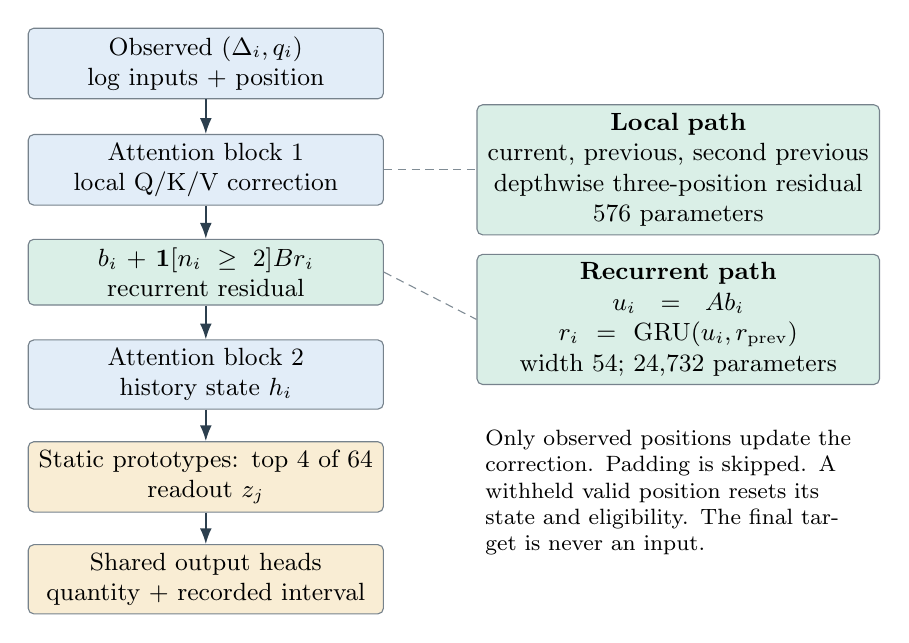
\begin{tikzpicture}[font=\small,>=Latex,
 box/.style={draw=ink!65,rounded corners=2pt,align=center,minimum height=8mm,text width=43mm,inner sep=3pt},
 flow/.style={->,draw=ink,semithick}]
\node[box,fill=enc] (input) at (0,0) {Observed $(\Delta_i,q_i)$\\log inputs + position};
\node[box,fill=enc] (first) at (0,-1.35) {Attention block 1\\local Q/K/V correction};
\node[box,fill=hist] (res) at (0,-2.65) {$b_i+\mathbf{1}[n_i\geq2]Br_i$\\recurrent residual};
\node[box,fill=enc] (second) at (0,-3.95) {Attention block 2\\history state $h_i$};
\node[box,fill=head] (proto) at (0,-5.25) {Static prototypes: top 4 of 64\\readout $z_j$};
\node[box,fill=head] (heads) at (0,-6.55) {Shared output heads\\quantity + recorded interval};
\foreach \a/\b in {input/first,first/res,res/second,second/proto,proto/heads}
 \draw[flow] (\a) -- (\b);
\node[box,text width=49mm,fill=hist] (local) at (6,-1.35) {\textbf{Local path}\\current, previous, second previous\\depthwise three-position residual\\576 parameters};
\node[box,text width=49mm,fill=hist] (gru) at (6,-3.25) {\textbf{Recurrent path}\\$u_i=A b_i$\\$r_i=\mathrm{GRU}(u_i,r_{\rm prev})$\\width 54; 24,732 parameters};
\node[align=left,text width=49mm,font=\footnotesize] at (6,-5.45) {Only observed positions update the correction. Padding is skipped. A withheld valid position resets its state and eligibility. The final target is never an input.};
\draw[densely dashed,draw=ink!60] (first.east) -- (local.west);
\draw[densely dashed,draw=ink!60] (res.east) -- (gru.west);
\end{tikzpicture}
\caption{CNN+GRU54 in \method. The local correction operates within the first attention block; the recurrent correction operates between blocks. Prototype retrieval and the two output heads follow the encoder. The correction paths contain 25,308 parameters in total.}
\label{fig:architecture}
\Description{A vertical causal encoder pipeline with enlarged local and recurrent correction modules to its right.}
\end{figure}

\subsection{Local and Recurrent History Correction}
For a projected query, key, or value sequence $X$, the local path computes
\begin{equation}
 \widetilde X_i=X_i+\sum_{\ell=0}^{2}a_{i\ell}\,\kappa^X_\ell\odot X_{s_\ell(i)}.
 \label{eq:local}
\end{equation}
Here $s_0(i)=i$, and $s_1(i),s_2(i)$ are the preceding observed positions in the same correction segment. The mask $a_{i\ell}$ indicates that the corresponding position exists. Each $\kappa^X_\ell\in\mathbb{R}^{64}$ acts channelwise. Applying this three-position operation to queries, keys, and values uses $3\times3\times64=576$ parameters. The operation permits nearby observed states to alter the attention inputs without replacing the attention layer itself.

The recurrent path projects the first-block output into a 54-dimensional state:
\begin{equation}
 u_i=A b_i,\qquad r_i=\mathrm{GRU}(u_i,r_{\mathrm{prev}}),\qquad
 \widetilde b_i=b_i+\mathbf{1}[n_i\geq2]B r_i.
 \label{eq:recurrent}
\end{equation}
The GRU follows the gated recurrent formulation~\cite{cho2014gru}; $A$ and $B$ are bias-free projections, and $n_i$ counts observed events in the current correction segment. The residual uses the state \emph{after} processing event $i$. The recurrent path has 24,732 parameters, including its projections. Its state width is independent of the number of observed events.

Padding neither updates the GRU nor advances the observation count. A valid but withheld position resets the correction state and its eligibility masks. This reset concerns the correction path; it does not change the causal attention mask into a segment-reset mask. The local kernels and recurrent output projection $B$ are initialized to zero. Thus the correction initially leaves the shared encoder computation unchanged, while its input and recurrent parameters can still be learned.

Algorithm~\ref{alg:history-correction} collects these operations for one input sequence. Local corrections read the original projected values, while the recurrent residual uses the state after the current observation. Zero initialization of the local kernels and $B$ occurs once before training, rather than at each forward pass.

\begin{algorithm}[H]
\caption{Causal local and recurrent history correction}
\label{alg:history-correction}
\small
\begin{algorithmic}[1]
\Require Observed-prefix embeddings $E$; valid and observed masks $v,o$;
\Statex \hspace{\algorithmicindent} causal attention mask $\mathcal A$. Withheld target values are excluded.
\Ensure Encoder state $h_j$ at the last observed position $j=\max\{i:o_i=1\}$.
\State Construct $s_\ell(i)$ and $a_{i\ell}$ from observed positions.
\Statex \hspace{\algorithmicindent} Skip padding; reset predecessors at valid but unobserved positions.
\State $(Q,K,V)\gets\operatorname{ProjectQKV}(\operatorname{LayerNorm}(E))$
\For{$X\in\{Q,K,V\}$}
    \State $\widetilde X\gets X$
    \For{each observed position $i$}
        \State $\widetilde X_i\gets X_i+\sum_{\ell=0}^{2}a_{i\ell}\,\kappa^X_\ell\odot X_{s_\ell(i)}$
    \EndFor
\EndFor
\State $b\gets\operatorname{CompleteBlock1}(E,\widetilde Q,\widetilde K,\widetilde V;\mathcal A)$
\Statex \hspace{\algorithmicindent} Retain persistent entries, attention and feed-forward residuals.
\State $\widetilde b\gets b$; $r\gets0$; $n\gets0$
\For{each position $i$ in sequence order}
    \If{$v_i=0$} \State \textbf{continue} \EndIf
    \If{$o_i=0$}
        \State $r\gets0$; $n\gets0$
        \State \textbf{continue}
    \EndIf
    \State $r\gets\operatorname{GRU}(A b_i,r)$
    \State $n\gets n+1$
    \If{$n\geq2$}
        \State $\widetilde b_i\gets b_i+B r$
    \EndIf
\EndFor
\State $h\gets\operatorname{Block2}(\widetilde b;\mathcal A)$
\State \Return $h_j$
\end{algorithmic}
\end{algorithm}

The correction states are maintained separately for each input sequence. Resetting them leaves the causal attention mask and persistent entries unchanged. The returned state is passed to prototype retrieval and the forecasting heads.

\paragraph{What the controls isolate.}
The correction-removal variant bypasses both optional paths. The current-only control retains their parameter shapes, initialization, and observation-count masks, but removes direct reads of earlier positions. In Eq.~\eqref{eq:local}, the three bases become $X_i$, $\tanh(X_i)$, and $\GELU(X_i)$, with the original one-, two-, and three-observation eligibility. For the recurrent component, the current-only control starts from zero at each position and applies two GRU updates using the same current input $u_i$. Its projected output is used only when $n_i\geq2$.

The full and current-only paths both contain 25,308 active correction parameters. Their computations nevertheless differ: the current-only control uses nonlinear bases and repeated current-input updates. It also receives $b_i$, which already summarizes a prefix through attention. Consequently, this comparison isolates a particular explicit history path against a current-position path; it does not compare a model with history against one without history, or identify the effect of a single lag in isolation.

\subsection{Static Prototype Retrieval}
After the encoder, a learned bank $M=\{m_k\}_{k=1}^{64}$ supplies a residual to the last observed state $h_j$. Each slot $m_k\in\mathbb{R}^{64}$ serves as both key and value: its normalized vector is used for scoring, and its raw vector is added to the readout. The slots are fitted with the rest of the model and are not written with observed events at inference time.

Let $\Nrm(x)=x/\max(\|x\|_2,\epsilon)$ and let $S_j$ contain the four highest-scoring slots. The mean baseline uses cosine scores $s_{jk}=\Nrm(h_j)^\top\Nrm(m_k)$ and uniform weights. The weighted variant retains these scores but applies a softmax within the selected four:
\begin{equation}
 z_j=h_j+\sum_{k\in S_j}\alpha_{jk}m_k,\qquad
 \alpha_{jk}=\frac{\exp(s_{jk})}{\sum_{v\in S_j}\exp(s_{jv})}.
 \label{eq:readout}
\end{equation}
Mean retrieval instead sets $\alpha_{jk}=1/4$. Neither variant introduces additional query parameters.

The two learned-query variants receive summaries of the most recent 32 observed positions in the current correction segment, including the current event. Time summaries use standardized $\log(\Delta/s)$; quantity summaries use standardized $\log(1+q)$, with moments computed from training observations. Each four-dimensional view contains the latest value, mean, population standard deviation, and difference between the latest two eligible values. Nonpositive gaps are excluded from time summaries, whereas zero quantities are retained. The standard deviation and difference require two eligible observations; unavailable summaries are zero. Denote the resulting views by $\phi_t$ and $\phi_q$.

The fixed split-query rule forms
\begin{align}
 v_t&=h_j+\phi_t W_t, & v_q&=h_j+\phi_q W_q,\\
 s^{\mathrm{fixed}}_{jk}
 &=\tfrac12\Nrm(v_t)^\top\Nrm(m_k)
   +\tfrac12\Nrm(v_q)^\top\Nrm(m_k).
 \label{eq:fixed}
\end{align}
The two $4\times64$ projections contain 512 parameters. A budget-matched general-query control uses the same eight summaries, with
\begin{equation}
 v_g=h_j+\tfrac12[\phi_t,\phi_q]W_g,\qquad
 s^{\mathrm{general}}_{jk}=\Nrm(v_g)^\top\Nrm(m_k),
 \label{eq:generic}
\end{equation}
where $W_g\in\mathbb{R}^{8\times64}$. Both variants use Eq.~\eqref{eq:readout}, temperature one, and zero-initialized query projections. Figure~\ref{fig:retrieval} highlights the difference: separate normalization before score averaging versus normalization after the two views have been combined.

\begin{figure}[t]
\centering
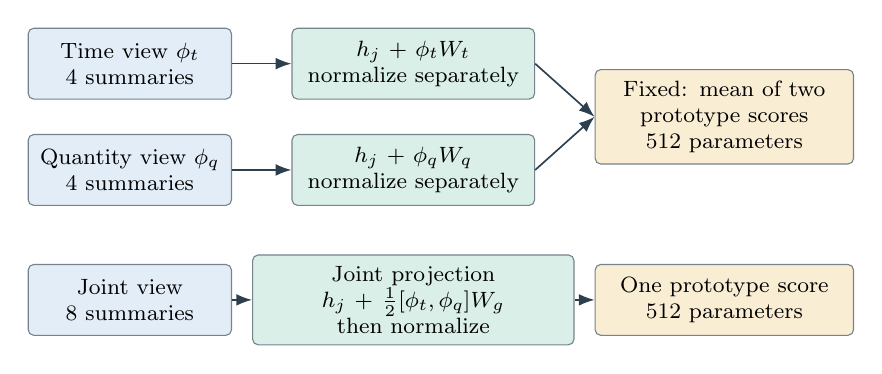
\begin{tikzpicture}[font=\footnotesize,>=Latex,
 b/.style={draw=ink!65,rounded corners=2pt,align=center,inner sep=4pt,minimum height=9mm},
 a/.style={->,semithick,draw=ink}]
\node[b,fill=enc,text width=23mm] (t) at (0,0) {Time view $\phi_t$\\4 summaries};
\node[b,fill=enc,text width=23mm] (q) at (0,-1.35) {Quantity view $\phi_q$\\4 summaries};
\node[b,fill=hist,text width=28mm] (tn) at (3.6,0) {$h_j+\phi_tW_t$\\normalize separately};
\node[b,fill=hist,text width=28mm] (qn) at (3.6,-1.35) {$h_j+\phi_qW_q$\\normalize separately};
\node[b,fill=head,text width=30mm] (f) at (7.55,-.675) {Fixed: mean of two\\prototype scores\\512 parameters};
\draw[a] (t) -- (tn); \draw[a] (q) -- (qn);
\draw[a] (tn.east) -- (f.west); \draw[a] (qn.east) -- (f.west);
\node[b,fill=enc,text width=23mm] (joint) at (0,-3) {Joint view\\8 summaries};
\node[b,fill=hist,text width=38mm] (g) at (3.6,-3) {Joint projection\\$h_j+\tfrac12[\phi_t,\phi_q]W_g$\\then normalize};
\node[b,fill=head,text width=30mm] (gs) at (7.55,-3) {One prototype score\\512 parameters};
\draw[a] (joint) -- (g); \draw[a] (g) -- (gs);

\end{tikzpicture}
\caption{The matched retrieval comparison. Both rules select four of 64 prototypes and use softmax weights. The fixed rule constrains two normalized views to equal score contributions; the general query learns a joint projection before normalization.}
\label{fig:retrieval}
\Description{Separate normalized time and quantity queries compared with a joint normalized query, each with 512 additional parameters.}
\end{figure}

The fixed score also has a concatenated dot-product expression:
\begin{equation}
 \tfrac12[\Nrm(v_t),\Nrm(v_q)]^\top[\Nrm(m_k),\Nrm(m_k)].
\end{equation}
The comparison tests separate query normalization and fixed score mixing. The comparisons share an architecture, not fitted encoder or prototype values: every arm is trained end to end.

\subsection{Shared Output Heads and Training Objective}
The quantity head predicts in log space and is evaluated in raw units:
\begin{equation}
 \widehat\ell_j=\softplus(w_q^\top z_j+b_q),\qquad
 \widehat q_{j+1}=\exp(\widehat\ell_j)-1.
\end{equation}
No inverse training-set standardization is applied. The time head gives
\begin{equation}
 \mu_j=w_\mu^\top z_j+b_\mu,\qquad
 \sigma_j=10^{-3}+\softplus(w_\sigma^\top z_j+b_\sigma).
\end{equation}
For a dataset scale $s>0$, let $T=s\exp(\mu_j+\sigma_j\varepsilon)$ with $\varepsilon\sim\mathcal N(0,1)$ and $F_j(x)=\Phi((\log(x/s)-\mu_j)/\sigma_j)$. The recorded interval is $D=\max(1,\operatorname{round}T)$, so its probability mass is
\begin{equation}
 p_j(d)=
 \begin{cases}
 F_j(1.5),& d=1,\\
 F_j(d+0.5)-F_j(d-0.5),& d\geq2.
 \end{cases}
 \label{eq:time}
\end{equation}
For Instacart, the recorded interval is capped at 30 days: the interior-bin rule applies for $2\leq d<30$, and $p_j(30)=1-F_j(29.5)$. Training minimizes the sum of recorded-time negative log-likelihood and squared log-quantity error,
\begin{equation}
 \mathcal L=-\log p_j(D_{j+1})+
   \bigl(\widehat\ell_j-\log(1+q_{j+1})\bigr)^2.
\end{equation}
The quantity weight is one, with no extra large-quantity loss term. All compared arms use these heads and this objective.

\section{Experimental Design}
\subsection{Datasets and Model Selection}
Taxi, Intermittent, and RAF Spare Parts form the core study. Instacart provides a supplementary architecture comparison. Table~\ref{tab:data} gives the eligible target populations and input windows. Lookback is measured in each dataset's native time bins. The inclusive window ends at the last observed event; the target is appended before truncation to the sequence cap, which includes that target. Large-quantity thresholds are fixed from the training data. Appendix~\ref{app:data-characteristics} gives the event definitions and training distributions; Appendix~\ref{app:lag} examines associations across observed-event lags.

\begin{table}[t]
\caption{Target populations and sequence construction. $q_{\rm large}$ is a strict lower bound for the large-quantity subset. Scale $s$ is used by the time distribution.}
\label{tab:data}
\centering\small
\setlength{\tabcolsep}{4pt}
\begin{tabular}{@{}lrrrllr@{}}
\toprule
Dataset & Training & Validation & Cap & Lookback & $q_{\rm large}$ & $s$\\
\midrule
Taxi & 38,393 & 8,268 & 256 & 168 hours & $3449$ & 1\\
Intermittent & 393,824 & 86,285 & 256 & 520 weeks & $187$ & 3\\
RAF & 25,779 & 6,690 & 84 & 84 months & $200$ & 6\\
Instacart & 1,991,192 & 503,733 & 64 & 52 days & $35$ & 7\\
\bottomrule
\end{tabular}
\end{table}

The representative experiments use AdamW~\cite{loshchilov2019adamw}, learning rate $10^{-3}$, weight decay 0.01, batch size 128, and gradient clipping at one. Training lasts at least 40 and at most 300 epochs, with patience 40. Each fit retains the first strictly improving finite minimum of overall raw-quantity RMSE on the full validation set. Ties retain the earlier checkpoint. This rule is shared by the earlier common-head panel, the completed MLP8 study, and the new comparisons; neither timing likelihood nor large-quantity error changes the selected epoch.

We evaluate quantity RMSE, quantity MAE, and recorded-time NLL on all validation targets and on the large-quantity subset. All six metrics come from that one checkpoint. Three-seed summaries use the arithmetic mean and sample standard deviation. Time scores are interpreted within a dataset, since the recorded units and distributions differ. Appendix~\ref{app:strata} specifies partitions by quantity and usable history, including how their errors contribute to an aggregate difference.

\subsection{Comparisons and Their Scope}
\paragraph{Earlier common-head comparison.}
We retain the completed comparison of TitanTPP-MLP4 with RMTPP, NHP, THP, SAHP, S2P2, and AttNHP~\cite{du2016rmtpp,mei2017nhp,zuo2020thp,zhang2020sahp,chang2025s2p2,yang2022anhp}. These are adaptations to numerical event inputs and the common quantity and recorded-time heads, rather than reproductions of native marked-event likelihood comparisons. The seven models, four datasets, and seeds 42, 52, and 62 give 84 fits. Their frozen contracts agree with the target populations, observed windows, loss, optimizer, and selection rule above. Each metric retains its run's selected checkpoint.

The historical TitanTPP model uses eight width-four MLP correction branches, with 6,144 nominal correction parameters. We label it MLP4 to distinguish it from the MLP8 ablation and CNN+GRU54. Software environments, initialization, and checkpoints differ across the historical and current campaigns; matching the task does not make their training trajectories equivalent. The historical panel establishes where MLP4 stands among the tested encoder adaptations, while the later controls address the correction mechanism.

Two encoder adaptations warrant further detail. S2P2 uses two width-64 layers with state size 16, complex dynamics, backward zero-order hold, and relative-time inputs. Its affine-doubling recurrence takes $O(L\log L)$ work for a length-$L$ sequence. AttNHP uses two width-64 layers, one attention head, and 16 time features. Both expose the state immediately after the last observed event to the common heads; neither receives the target event time. These adaptations do not support claims about the original models' native likelihoods or computational efficiency. Two nonlearned quantity references repeat the last observed quantity or average the quantities in the same available input window. They do not supply timing distributions.

\paragraph{Completed MLP8 correction study.}
The initial study crosses prototype removal/addition ($P_0/P_1$) with correction removal/addition ($H_0/H_1$), giving a $2\times2$ comparison. It places an MLP correction between the first and second attention blocks, with no local Q/K/V correction; prototype retrieval follows the second block. Thus it differs from both correction paths in CNN+GRU54. Eight bias-free branches each map the concatenated current and immediately preceding observed states through $128\!\to\!8\!\to\!64$, and their outputs are averaged. The branches become eligible after more than 1, 2, 4, 8, 16, 32, 64, or 128 observations. These are eligibility thresholds, not eight different history lags.

The correction contains 12,288 parameters; the 64-slot prototype bank contains 4,096. Two additional controls test alternatives to these components. $P_1H_C$ replaces the correction with eight current-state branches of width 12, matching its parameter count. $P_FH_1$ replaces the prototype residual with a bias-free $64\!\to\!32\!\to\!64$ feed-forward residual, also using 4,096 parameters. All six arms retain the backbone's persistent attention entries. The six arms, three datasets, and seeds 42, 52, and 62 produce 54 completed fits.

These budget controls have limits. The feed-forward substitute differs in activation and initialization from prototype retrieval. Equal parameter counts do not imply equal computation. On RAF, the sequence cap prevents the eighth MLP branch from becoming eligible, leaving seven potentially active branches. These details constrain what can be attributed to the nominal budgets.

\paragraph{Representative correction and retrieval studies.}
CNN+GRU54 is compared with correction removal and the current-only control on each core dataset and seed: 27 fits. The retrieval comparison adds weighted, fixed, and general-query variants, with the nine full-correction models reused as the mean baseline. This requires 27 further fits, rather than a second training of the same mean models. The matched general query has 512 added parameters; it is distinct from the 521-parameter control used in the earlier exploratory retrieval pilot.

For a dataset and seed, all comparison arms run on the same GPU and software environment. Taxi and RAF are assigned to RTX 5080; Intermittent to RTX 5090. A preliminary implementation check compared CNN+GRU54 with mean retrieval on RTX 5080: 83 bitwise checks covered initialization, synthetic sequences, and the first three updates on a shared Taxi training batch. This establishes a limited implementation baseline, not equivalence of past training trajectories or checkpoints obtained on another GPU.

On Instacart, the supplementary study compares MLP8, MLP12, and CNN+GRU54 across the same three seeds, adding nine fits. It asks about architecture behavior on a fourth dataset; it does not replace the correction or retrieval controls. Together, these studies specify 63 new fits. Their completed comparisons will determine the representative model's evidence, separately from the MLP4 and MLP8 findings below.

\paragraph{Decision criteria and computational cost.}
The correction criterion requires the full model to have lower overall quantity RMSE than both controls in every seed on the same two or more core datasets. The fixed-retrieval criterion requires corresponding improvements over mean, weighted, and the general-query control. These are descriptive consistency criteria, not significance tests.

Retrieval must also meet a predeclared cost bound relative to mean retrieval on the same GPU. With batch 128, sequence lengths 64 and 256, five warm-up iterations and twenty measured iterations, the allowed increases are 20\% for inference time, 30\% for training-step time, and 20\% for peak allocation. Both lengths must pass. Results from arms above these bounds remain part of the comparison.

\section{Results}
\subsection{Overall Performance in the Earlier Common-Head Study}
Table~\ref{tab:external-legacy} reports the completed four-dataset comparison. On Taxi and Intermittent, TitanTPP-MLP4 has lower quantity MAE and RMSE than all six encoder adaptations in every paired seed. These are 36 model--dataset--seed comparisons for each quantity metric. Relative to RMTPP, which has the lowest mean quantity errors among the six alternatives on both datasets, mean RMSE is lower by 15.85\% on Taxi and 34.39\% on Intermittent; mean MAE is lower by 10.13\% and 21.72\%, respectively.

\begin{table}[p]
\caption{Historical development-validation comparison with numerical-input, common-head adaptations of the external encoders. Values are mean $\pm$ sample standard deviation over seeds 42, 52, and 62; all three metrics use the same RMSE-selected checkpoint within each run. TitanTPP (MLP4) denotes the earlier eight-branch, width-four correction (6,144 parameters), not CNN+GRU54. Bold marks the lowest mean in each dataset and metric within this panel.}
\label{tab:external-legacy}\centering\small
\begin{tabular}{lrrr}
\toprule
Model & Quantity MAE & Quantity RMSE & Time NLL\\
\midrule
\multicolumn{4}{l}{\textit{Taxi}}\\
TitanTPP (MLP4) & $\mathbf{25.6237\pm0.8320}$ & $\mathbf{79.7111\pm2.8260}$ & $1.0387\pm0.2843$\\
RMTPP & $28.5124\pm0.6344$ & $94.7283\pm3.4006$ & $1.5798\pm0.9400$\\
THP & $32.4095\pm0.8144$ & $107.5977\pm4.5040$ & $0.6629\pm0.0174$\\
NHP & $94.2694\pm1.8752$ & $318.8148\pm5.3011$ & $\mathbf{0.6516\pm0.0021}$\\
SAHP & $34.2260\pm0.4539$ & $120.5273\pm1.9996$ & $0.6848\pm0.0146$\\
S2P2 & $33.0231\pm0.5569$ & $106.3540\pm1.9135$ & $0.6658\pm0.0242$\\
AttNHP & $35.9811\pm1.6088$ & $127.1290\pm8.9919$ & $0.6876\pm0.0194$\\
\midrule
\multicolumn{4}{l}{\textit{Intermittent}}\\
TitanTPP (MLP4) & $\mathbf{0.7005\pm0.0541}$ & $\mathbf{1.6730\pm0.0819}$ & $0.4971\pm0.2095$\\
RMTPP & $0.8949\pm0.0494$ & $2.5499\pm0.1604$ & $0.2748\pm0.0047$\\
THP & $0.8993\pm0.0661$ & $2.7534\pm0.1784$ & $0.2911\pm0.0045$\\
NHP & $4.5188\pm0.1706$ & $12.8755\pm1.0405$ & $0.4613\pm0.0969$\\
SAHP & $1.8619\pm0.0899$ & $7.0298\pm0.7673$ & $0.3448\pm0.0138$\\
S2P2 & $0.9359\pm0.0086$ & $2.5758\pm0.0766$ & $\mathbf{0.2349\pm0.0189}$\\
AttNHP & $1.0413\pm0.0938$ & $3.0799\pm0.2982$ & $0.2946\pm0.0569$\\
\midrule
\multicolumn{4}{l}{\textit{RAF}}\\
TitanTPP (MLP4) & $9.2506\pm0.0855$ & $\mathbf{33.9507\pm0.0588}$ & $3.5446\pm0.0669$\\
RMTPP & $\mathbf{9.1362\pm0.0557}$ & $34.5503\pm0.2506$ & $3.5191\pm0.1463$\\
THP & $9.3014\pm0.1819$ & $34.7445\pm0.3204$ & $3.3928\pm0.0187$\\
NHP & $9.1793\pm0.0882$ & $36.2731\pm0.3186$ & $\mathbf{3.3889\pm0.0556}$\\
SAHP & $9.2332\pm0.0209$ & $35.4193\pm0.2130$ & $3.7415\pm0.0745$\\
S2P2 & $9.2730\pm0.0517$ & $33.9947\pm0.1261$ & $3.4187\pm0.0284$\\
AttNHP & $9.1917\pm0.0434$ & $34.8766\pm0.0676$ & $3.9707\pm0.0609$\\
\midrule
\multicolumn{4}{l}{\textit{Instacart}}\\
TitanTPP (MLP4) & $3.9916\pm0.0026$ & $5.8827\pm0.0048$ & $2.8071\pm0.0041$\\
RMTPP & $\mathbf{3.9852\pm0.0052}$ & $5.8775\pm0.0213$ & $2.8051\pm0.0048$\\
THP & $4.0013\pm0.0025$ & $5.8582\pm0.0253$ & $2.8056\pm0.0016$\\
NHP & $4.4923\pm0.0304$ & $6.7613\pm0.0538$ & $2.8132\pm0.0080$\\
SAHP & $3.9979\pm0.0099$ & $5.8776\pm0.0067$ & $2.8018\pm0.0013$\\
S2P2 & $3.9987\pm0.0063$ & $\mathbf{5.8523\pm0.0150}$ & $\mathbf{2.7970\pm0.0014}$\\
AttNHP & $3.9958\pm0.0021$ & $5.8648\pm0.0194$ & $2.8080\pm0.0028$\\
\bottomrule
\end{tabular}
\end{table}

The result is narrower on RAF. MLP4 has the lowest mean RMSE, but its advantage over S2P2 is only 0.13\%, with improvements in two of three paired seeds. RMTPP has lower mean MAE. On Instacart, S2P2 has the lowest mean RMSE and timing NLL, while RMTPP has the lowest mean MAE. MLP4 has 0.52\% higher mean RMSE than S2P2, and both S2P2 and AttNHP have lower RMSE in all three paired seeds. These differences rule out a uniform quantity ranking across the four datasets.

Timing provides a further distinction. NHP has the lowest mean time NLL on Taxi and RAF, and S2P2 does so on Intermittent and Instacart. For example, MLP4's Taxi NLL is 1.0387, compared with 0.6516 for NHP; on Intermittent, it is 0.4971, compared with 0.2349 for S2P2. The quantity advantage therefore coexists with worse timing scores at the quantity-selected checkpoints.

Table~\ref{tab:external-simple} puts these quantity results alongside the two nonlearned rules. MLP4 has lower RMSE than both on all four datasets. On Intermittent, however, repeating the last quantity gives lower MAE, 0.5647 versus 0.7005, while its RMSE is 1.7078 versus 1.6730. This disagreement between MAE and RMSE is material: outperforming the learned encoders does not mean that the model improves every measure over a simple rule.

\begin{table}[t]
\caption{Historical validation comparison with nonlearned quantity rules on the same targets and observed windows. TitanTPP (MLP4) entries are three-seed means; deterministic rules have one result, no seed standard deviation, and no duration likelihood.}
\label{tab:external-simple}\centering\small
\begin{tabular}{llrr}
\toprule
Dataset & Predictor & MAE & RMSE\\
\midrule
Taxi & TitanTPP (MLP4) & 25.6237 & 79.7111\\
 & Last quantity & 41.1951 & 134.3931\\
 & Window mean & 120.3771 & 368.7843\\
\midrule
Intermittent & TitanTPP (MLP4) & 0.7005 & 1.6730\\
 & Last quantity & 0.5647 & 1.7078\\
 & Window mean & 4.5537 & 13.7821\\
\midrule
RAF & TitanTPP (MLP4) & 9.2506 & 33.9507\\
 & Last quantity & 11.3136 & 44.5742\\
 & Window mean & 10.8564 & 36.8499\\
\midrule
Instacart & TitanTPP (MLP4) & 3.9916 & 5.8827\\
 & Last quantity & 4.9674 & 7.3473\\
 & Window mean & 4.0507 & 5.9030\\
\bottomrule
\end{tabular}
\end{table}


These results describe the archived MLP4 variant under common heads. They establish neither the benefit of the CNN+GRU correction nor the effect of changing its retrieval rule. We next examine the separate MLP8 ablation to distinguish the correction and prototype contributions.

\subsection{Quantity Gains in the Completed MLP8 Study}
Table~\ref{tab:rmse} reports the complete six-arm quantity comparison. Adding the MLP correction reduces overall RMSE in all 18 paired comparisons: three datasets, three seeds, and two prototype settings. Without prototypes, the reductions in the means are 13.04\% on Taxi, 9.01\% on Intermittent, and 0.77\% on RAF. With prototypes, the corresponding reductions are 14.11\%, 3.28\%, and 0.85\%. The direction is consistent, but the magnitude is strongly dataset-dependent.

\begin{table}[t]
\caption{Completed MLP8 study: overall validation quantity RMSE (mean $\pm$ sample SD over three seeds; lower is better). Bold marks the lowest mean within each dataset. These are not CNN+GRU54 results.}
\label{tab:rmse}
\centering\small
\setlength{\tabcolsep}{6pt}
\begin{tabular}{@{}lccc@{}}
\toprule
Arm & Taxi & Intermittent & RAF\\
\midrule
$P_0H_0$ & \pmval{88.977}{0.501} & \pmval{1.777}{0.065} & \pmval{34.242}{0.147}\\
$P_1H_0$ & \pmval{90.509}{0.521} & \pmval{1.721}{0.045} & \pmval{34.230}{0.127}\\
$P_0H_1$ & $\mathbf{77.377}\,{\scriptstyle\pm}\,1.822$ & $\mathbf{1.617}\,{\scriptstyle\pm}\,0.009$ & \pmval{33.979}{0.045}\\
$P_1H_1$ & \pmval{77.735}{0.681} & \pmval{1.664}{0.009} & $\mathbf{33.938}\,{\scriptstyle\pm}\,0.071$\\
$P_FH_1$ & \pmval{79.255}{1.230} & \pmval{1.759}{0.124} & \pmval{34.125}{0.074}\\
$P_1H_C$ & \pmval{88.846}{1.267} & \pmval{1.728}{0.061} & \pmval{34.273}{0.327}\\
\bottomrule
\end{tabular}
\end{table}

The parameter controls provide a more selective result. $P_1H_1$ beats both $P_FH_1$ and $P_1H_C$ in all three seeds on Taxi and RAF. On Intermittent, it beats each control in only two of three seeds. Thus the MLP8 study satisfies its two-dataset consistency criterion, while leaving an exception on Intermittent. The large Taxi gap against $P_1H_C$ is compatible with useful explicit previous-state input in this MLP architecture; the control does not establish which part of the CNN+GRU path would account for such an effect.

Prototype addition yields a different pattern. With the correction already present, $P_1H_1$ has 0.46\% higher mean RMSE than $P_0H_1$ on Taxi and 2.92\% higher RMSE on Intermittent. On RAF it improves the mean by 0.12\%. The completed evidence therefore favors explicit correction more consistently than prototype addition. Choosing a different best variant for each dataset would conceal this distinction and would not define a single representative model.

\subsection{Timing, Large Quantities, and Cost in the MLP8 Study}
Quantity gains are not uniform gains across outputs. On Taxi, adding correction raises overall time NLL from 0.818 to 1.253 without prototypes and from 0.725 to 1.229 with prototypes. These are increases of 53.17\% and 69.64\% in the means; timing NLL worsens in every seed under both settings. The checkpoints were selected for quantity RMSE, so this is a tradeoff at the quantity-selected model rather than a comparison of separately optimized timing checkpoints.

Large-quantity behavior also qualifies the overall result. The Taxi full model has large-quantity RMSE 376.660, compared with 366.709 for its feed-forward prototype substitute, despite lower overall RMSE. On RAF, adding correction slightly reduces overall RMSE but increases large-quantity MAE by 1.27\% without prototypes and 0.94\% with prototypes. Its large-quantity time NLL rises by 3.64\% and 3.85\%, respectively. The large subsets contain only 79 Taxi targets and 50 RAF targets, compared with 1,141 on Intermittent. Appendix~\ref{app:metrics} retains all six metrics, including these unfavorable outcomes.

The historical technical checks do not show that prototype retrieval is cheaper than its parameter-matched substitute. On RTX 5080, the measured step time for $P_1H_1$ is 36.46\,ms versus 25.34\,ms for $P_FH_1$ at length 256, and 14.15\,ms versus 11.49\,ms at length 84. On RTX 5090 at length 256, the corresponding times are 23.11 and 17.74\,ms. These checks use the median of three synthetic optimizer steps, without discarded warm-up, and include gradient-copy and verification work. They are limited technical measurements, not pure throughput or inference benchmarks, and do not implement the new retrieval cost protocol.

\subsection{Evidence Available for the Representative Architecture}
The CNN+GRU correction and matched retrieval comparisons do not yet have completed results in the evidence used here. Their implementation and experimental controls are specified in Sections 3 and 4, but the MLP results cannot establish their effects.

The archived observation of 8 October 2026, 14:38 KST contains one completed Instacart fit: MLP8, seed 52, on RTX 5090. It selected epoch 15 and stopped after epoch 55, with overall quantity RMSE 5.884, MAE 3.994, and time NLL 2.812. For the 6,036 large-quantity targets, the same checkpoint gives RMSE 24.665, MAE 22.088, and time NLL 2.900. This is a single-fit observation, not a three-seed architecture comparison; final collection of the complete stage remains outstanding. It cannot rank MLP8, MLP12, and CNN+GRU54.

\section{Discussion}
The completed MLP8 study gives a specific empirical motivation for explicit correction. Quantity RMSE improves consistently when the MLP path is added, and the full model beats the two budget controls in every seed on two datasets. At the same time, prototype addition is not consistently helpful, and the largest correction gains coincide with a timing penalty. These results argue for separating the two mechanisms and for keeping timing and large-quantity errors visible alongside the primary metric.

The representative architecture changes the correction mechanism substantially. Its local operation reads three observed positions, while its GRU carries a recurrent state across the observed prefix. A successful full-versus-current-only comparison would support that combined path, not a claim that one preceding state alone explains the gain. Equal active parameter counts narrow the capacity explanation but do not remove differences in operations, depth, or optimization. Component-level attribution would require further controls.

The retrieval hypothesis is narrower still. Fixed split-query scoring can be expressed as a concatenated dot product. A benefit over the matched general query would support the tested separate-normalization constraint, not the invention of a fundamentally new memory mechanism. A benefit over mean alone would be insufficient, because both similarity weighting and general query learning are plausible alternatives. Earlier exploratory observations informed this hypothesis, making the new comparison a development study rather than independent confirmation.

The earlier common-head comparison supports a bounded performance claim for MLP4: lower quantity errors than the six tested encoder adaptations on Taxi and Intermittent, and a small RMSE advantage on RAF. On Instacart, it does not achieve the lowest RMSE. It does not rank the new CNN+GRU54 model, and it compares adapted encoders rather than the original native likelihood models.

All performance reported here comes from validation evidence used during research. An independently unexposed evaluation is not yet available. Three seeds and directional consistency describe the current evidence; they do not establish statistical significance or performance across all event-forecasting settings.

\section{Conclusion}
We examined explicit history correction within a causal attention model. The earlier MLP4 comparison shows strong quantity results on Taxi and Intermittent, but mixed results on RAF and Instacart. The MLP8 ablation finds consistent quantity improvements from correction across paired runs, together with timing and large-quantity costs. Its prototype results are less consistent. The CNN+GRU architecture and matched controls carry these observations into two focused questions: whether an explicit local and recurrent path adds value, and whether separate time and quantity queries improve prototype retrieval. Those comparisons, followed by an unexposed evaluation, will determine how far the present evidence extends.

\begin{thebibliography}{28}
\bibitem{bachlechner2021rezero}
Bachlechner, T., Majumder, B. P., Mao, H., Cottrell, G., McAuley, J.: \href{https://proceedings.mlr.press/v161/bachlechner21a.html}{ReZero is all you need: fast convergence at large depth}. Proceedings of the Thirty-Seventh Conference on Uncertainty in Artificial Intelligence \textbf{161}, 1352--1361 (2021).

\bibitem{behrouz2025titans}
Behrouz, A., Zhong, P., Mirrokni, V.: \href{https://papers.nips.cc/paper_files/paper/2025/hash/a4ca07aa108036f80cbb5b82285fd4b1-Abstract-Conference.html}{Titans: Learning to Memorize at Test Time}. Advances in Neural Information Processing Systems 38, 125925--125962 (2025). \doi{10.52202/085713-3786}

\bibitem{chang2025s2p2}
Chang, Y., Boyd, A., Xiao, C., Kass-Hout, T., Bhatia, P., Smyth, P., Warrington, A.:
\href{https://arxiv.org/abs/2412.19634}{Deep continuous-time state-space models for marked event sequences}. In: Advances in Neural Information Processing Systems, vol. 38 (2025).

\bibitem{cho2014gru}
Cho, K., van Merri\"enboer, B., G\"ul\c{c}ehre, \c{C}., Bahdanau, D., Bougares, F., Schwenk, H., Bengio, Y.:
\href{https://arxiv.org/abs/1406.1078}{Learning phrase representations using RNN encoder--decoder for statistical machine translation}. In: EMNLP (2014).

\bibitem{croston1972forecasting}
Croston, J. D.: \href{https://link.springer.com/article/10.1057/jors.1972.50}{Forecasting and Stock Control for Intermittent Demands}. Journal of the Operational Research Society \textbf{23}(3), 289--303 (1972). \doi{10.1057/jors.1972.50}

\bibitem{draxler2025flextpp}
Draxler, F., Meng, Y., Nelson, K., Laskowski, L., Yang, Y., Karaletsos, T., et al.: \href{https://proceedings.nips.cc/paper_files/paper/2025/hash/a6c7515ac435277dc92b75a07bb2257c-Abstract-Conference.html}{Transformers for Mixed-type Event Sequences}. Advances in Neural Information Processing Systems 38, 127441--127473 (2025). \doi{10.52202/085713-3833}

\bibitem{du2016rmtpp}
Du, N., Dai, H., Trivedi, R., Upadhyay, U., Gomez-Rodriguez, M., Song, L.:
\href{https://doi.org/10.1145/2939672.2939875}{Recurrent marked temporal point processes: Embedding event history to vector}. In: KDD, pp. 1555--1564 (2016). \doi{10.1145/2939672.2939875}

\bibitem{gneiting2007proper}
Gneiting, T., Raftery, A. E.: \href{https://doi.org/10.1198/016214506000001437}{Strictly Proper Scoring Rules, Prediction, and Estimation}. Journal of the American Statistical Association \textbf{102}(477), 359--378 (2007). \doi{10.1198/016214506000001437}

\bibitem{hawkes1971spectra}
Hawkes, A. G.: \href{https://academic.oup.com/biomet/article-abstract/58/1/83/224809}{Spectra of some self-exciting and mutually exciting point processes}. Biometrika \textbf{58}(1), 83--90 (1971). \doi{10.1093/biomet/58.1.83}

\bibitem{he2016residual}
He, K., Zhang, X., Ren, S., Sun, J.: \href{https://openaccess.thecvf.com/content_cvpr_2016/html/He_Deep_Residual_Learning_CVPR_2016_paper.html}{Deep Residual Learning for Image Recognition}. Proceedings of the IEEE Conference on Computer Vision and Pattern Recognition, 770--778 (2016). \doi{10.1109/CVPR.2016.90}

\bibitem{houlsby2019adapters}
Houlsby, N., Giurgiu, A., Jastrzebski, S., Morrone, B., De Laroussilhe, Q., Gesmundo, A., et al.: \href{https://proceedings.mlr.press/v97/houlsby19a.html}{Parameter-Efficient Transfer Learning for NLP}. Proceedings of the 36th International Conference on Machine Learning \textbf{97}, 2790--2799 (2019).

\bibitem{hyndman2006accuracy}
Hyndman, R. J., Koehler, A. B.: \href{https://doi.org/10.1016/j.ijforecast.2006.03.001}{Another look at measures of forecast accuracy}. International Journal of Forecasting \textbf{22}(4), 679--688 (2006). \doi{10.1016/j.ijforecast.2006.03.001}

\bibitem{lample2019product}
Lample, G., Sablayrolles, A., Ranzato, M., Denoyer, L., J\'egou, H.:
\href{https://papers.neurips.cc/paper/9061-large-memory-layers-with-product-keys}{Large memory layers with product keys}. In: Advances in Neural Information Processing Systems, vol. 32 (2019).

\bibitem{loshchilov2019adamw}
Loshchilov, I., Hutter, F.:
\href{https://arxiv.org/abs/1711.05101}{Decoupled weight decay regularization}. In: ICLR (2019).

\bibitem{mei2017nhp}
Mei, H., Eisner, J.: \href{https://papers.nips.cc/paper_files/paper/2017/hash/6463c88460bd63bbe256e495c63aa40b-Abstract.html}{The Neural Hawkes Process: A Neurally Self-Modulating Multivariate Point Process}. Advances in Neural Information Processing Systems 30 (2017).

\bibitem{omi2019fully}
Omi, T., Ueda, N., Aihara, K.: \href{https://proceedings.neurips.cc/paper/2019/hash/39e4973ba3321b80f37d9b55f63ed8b8-Abstract.html}{Fully Neural Network based Model for General Temporal Point Processes}. Advances in Neural Information Processing Systems 32 (2019).

\bibitem{salinas2020deepar}
Salinas, D., Flunkert, V., Gasthaus, J., Januschowski, T.: \href{https://www.sciencedirect.com/science/article/pii/S0169207019301888}{DeepAR: Probabilistic forecasting with autoregressive recurrent networks}. International Journal of Forecasting \textbf{36}(3), 1181--1191 (2020). \doi{10.1016/j.ijforecast.2019.07.001}

\bibitem{shchur2020intensityfree}
Shchur, O., Bilo\v{s}, M., G\"{u}nnemann, S.: \href{https://openreview.net/forum?id=HygOjhEYDH}{Intensity-Free Learning of Temporal Point Processes}. International Conference on Learning Representations (2020).

\bibitem{shchur2021review}
Shchur, O., T\"{u}rkmen, A. C., Januschowski, T., G\"{u}nnemann, S.: \href{https://www.ijcai.org/proceedings/2021/623}{Neural Temporal Point Processes: A Review}. Proceedings of the Thirtieth International Joint Conference on Artificial Intelligence, 4585--4593 (2021). \doi{10.24963/ijcai.2021/623}

\bibitem{sukhbaatar2015memory}
Sukhbaatar, S., Szlam, A., Weston, J., Fergus, R.: \href{https://proceedings.neurips.cc/paper/2015/hash/8fb21ee7a2207526da55a679f0332de2-Abstract.html}{End-To-End Memory Networks}. Advances in Neural Information Processing Systems 28 (2015).

\bibitem{sukhbaatar2019memory}
Sukhbaatar, S., Grave, E., Lample, G., J\'egou, H., Joulin, A.:
\href{https://arxiv.org/abs/1907.01470}{Augmenting self-attention with persistent memory}. arXiv:1907.01470 (2019).

\bibitem{syntetos2005accuracy}
Syntetos, A. A., Boylan, J. E.: \href{https://www.sciencedirect.com/science/article/pii/S0169207004000792}{The accuracy of intermittent demand estimates}. International Journal of Forecasting \textbf{21}(2), 303--314 (2005). \doi{10.1016/j.ijforecast.2004.10.001}

\bibitem{teunter2011obsolescence}
Teunter, R. H., Syntetos, A. A., Babai, M. Z.: \href{https://www.sciencedirect.com/science/article/pii/S0377221711004437}{Intermittent demand: Linking forecasting to inventory obsolescence}. European Journal of Operational Research \textbf{214}(3), 606--615 (2011). \doi{10.1016/j.ejor.2011.05.018}

\bibitem{turkmen2021renewal}
T\"urkmen, A.C., Januschowski, T., Wang, Y., Cemgil, A.T.:
\href{https://doi.org/10.1371/journal.pone.0259764}{Forecasting intermittent and sparse time series: A unified probabilistic framework via deep renewal processes}. PLOS ONE 16(11), e0259764 (2021). \doi{10.1371/journal.pone.0259764}

\bibitem{vaswani2017attention}
Vaswani, A., Shazeer, N., Parmar, N., Uszkoreit, J., Jones, L., Gomez, A.N., Kaiser, \L{}., Polosukhin, I.:
\href{https://arxiv.org/abs/1706.03762}{Attention is all you need}. In: Advances in Neural Information Processing Systems, vol. 30 (2017).

\bibitem{yang2022anhp}
Yang, C., Mei, H., Eisner, J.:
\href{https://www.cs.jhu.edu/~jason/papers/yang+al.iclr22.pdf}{Transformer embeddings of irregularly spaced events and their participants}. In: ICLR (2022).

\bibitem{zhang2020sahp}
Zhang, Q., Lipani, A., Kirnap, O., Yilmaz, E.: \href{https://proceedings.mlr.press/v119/zhang20q.html}{Self-Attentive Hawkes Process}. Proceedings of the 37th International Conference on Machine Learning \textbf{119}, 11183--11193 (2020).

\bibitem{zuo2020thp}
Zuo, S., Jiang, H., Li, Z., Zhao, T., Zha, H.: \href{https://proceedings.mlr.press/v119/zuo20a.html}{Transformer Hawkes Process}. Proceedings of the 37th International Conference on Machine Learning \textbf{119}, 11692--11702 (2020).
\end{thebibliography}

\clearpage
\appendix
\renewcommand{\theHsection}{\Alph{section}}
\section{Full Validation Metrics for the MLP8 Study}
\label{app:metrics}
All entries in Table~\ref{tab:allmetrics} are means and sample standard deviations over seeds 42, 52, and 62. Each fit contributes metrics from its first minimum-overall-quantity-RMSE checkpoint. The large subsets use the strict training-derived thresholds in Table~\ref{tab:data}. Values are rounded to three decimals except for time NLLs below 0.001, which use scientific notation with the standard deviation on the line beneath the mean. No metric in this table comes from the representative CNN+GRU experiment.

\begin{table}[htbp]
\caption{Completed MLP8 study: all six validation metrics (mean $\pm$ sample SD). Lower is better in every column. The large-quantity subset is shown beside the full population rather than used for independent checkpoint selection.}
\label{tab:allmetrics}
\centering\scriptsize
\setlength{\tabcolsep}{3pt}
\renewcommand{\arraystretch}{1.1}
\begin{tabular}{@{}lrrrrrr@{}}
\toprule
 & \multicolumn{3}{c}{All targets} & \multicolumn{3}{c}{Large-quantity targets}\\
\cmidrule(lr){2-4}\cmidrule(l){5-7}
Arm & RMSE & MAE & Time NLL & RMSE & MAE & Time NLL\\
\midrule
\multicolumn{7}{l}{\textit{Taxi: 8,268 targets; 79 large}}\\
$P_0H_0$ & \pmval{88.977}{0.501} & \pmval{28.313}{0.096} & \pmval{0.818}{0.191} & \pmval{419.317}{53.142} & \pmval{336.399}{45.621} & \shortstack{$1.21\!\times\!10^{-30}$\\$\pm2.09\!\times\!10^{-30}$}\\
$P_1H_0$ & \pmval{90.509}{0.521} & \pmval{28.755}{0.453} & \pmval{0.725}{0.067} & \pmval{431.690}{19.168} & \pmval{346.009}{21.136} & \shortstack{$6.36\!\times\!10^{-17}$\\$\pm1.10\!\times\!10^{-16}$}\\
$P_0H_1$ & \pmval{77.377}{1.822} & \pmval{25.180}{0.491} & \pmval{1.253}{0.125} & \pmval{385.604}{27.258} & \pmval{311.795}{29.080} & \shortstack{$9.77\!\times\!10^{-78}$\\$\pm1.69\!\times\!10^{-77}$}\\
$P_1H_1$ & \pmval{77.735}{0.681} & \pmval{25.040}{0.146} & \pmval{1.229}{0.160} & \pmval{376.660}{10.552} & \pmval{296.101}{11.577} & \shortstack{$5.51\!\times\!10^{-62}$\\$\pm9.54\!\times\!10^{-62}$}\\
$P_FH_1$ & \pmval{79.255}{1.230} & \pmval{25.475}{0.205} & \pmval{1.155}{0.373} & \pmval{366.709}{26.906} & \pmval{287.777}{23.170} & \shortstack{$1.58\!\times\!10^{-43}$\\$\pm2.74\!\times\!10^{-43}$}\\
$P_1H_C$ & \pmval{88.846}{1.267} & \pmval{28.422}{0.295} & \pmval{1.001}{0.322} & \pmval{398.429}{29.267} & \pmval{314.315}{23.846} & \shortstack{$1.82\!\times\!10^{-25}$\\$\pm3.15\!\times\!10^{-25}$}\\
\midrule
\multicolumn{7}{l}{\textit{Intermittent: 86,285 targets; 1,141 large}}\\
$P_0H_0$ & \pmval{1.777}{0.065} & \pmval{0.751}{0.042} & \pmval{0.366}{0.016} & \pmval{8.121}{0.462} & \pmval{6.406}{0.382} & \pmval{0.035}{0.046}\\
$P_1H_0$ & \pmval{1.721}{0.045} & \pmval{0.735}{0.048} & \pmval{0.371}{0.050} & \pmval{8.000}{0.165} & \pmval{6.163}{0.145} & \shortstack{$1.32\!\times\!10^{-4}$\\$\pm2.28\!\times\!10^{-4}$}\\
$P_0H_1$ & \pmval{1.617}{0.009} & \pmval{0.669}{0.015} & \pmval{0.384}{0.041} & \pmval{7.510}{0.441} & \pmval{5.561}{0.283} & \pmval{0.004}{0.007}\\
$P_1H_1$ & \pmval{1.664}{0.009} & \pmval{0.722}{0.009} & \pmval{0.370}{0.059} & \pmval{7.711}{0.125} & \pmval{5.986}{0.290} & \pmval{0.016}{0.028}\\
$P_FH_1$ & \pmval{1.759}{0.124} & \pmval{0.745}{0.105} & \pmval{0.356}{0.068} & \pmval{8.911}{0.805} & \pmval{6.481}{0.575} & \pmval{0.387}{0.645}\\
$P_1H_C$ & \pmval{1.728}{0.061} & \pmval{0.710}{0.023} & \pmval{0.551}{0.350} & \pmval{8.315}{0.473} & \pmval{6.541}{0.402} & \pmval{9.908}{17.131}\\
\midrule
\multicolumn{7}{l}{\textit{RAF: 6,690 targets; 50 large}}\\
$P_0H_0$ & \pmval{34.242}{0.147} & \pmval{9.270}{0.057} & \pmval{3.592}{0.112} & \pmval{326.556}{6.460} & \pmval{279.427}{7.680} & \pmval{3.455}{0.150}\\
$P_1H_0$ & \pmval{34.230}{0.127} & \pmval{9.261}{0.062} & \pmval{3.596}{0.112} & \pmval{326.405}{6.068} & \pmval{279.348}{7.255} & \pmval{3.447}{0.145}\\
$P_0H_1$ & \pmval{33.979}{0.045} & \pmval{9.259}{0.099} & \pmval{3.554}{0.078} & \pmval{327.105}{1.589} & \pmval{282.972}{2.416} & \pmval{3.581}{0.220}\\
$P_1H_1$ & \pmval{33.938}{0.071} & \pmval{9.266}{0.092} & \pmval{3.552}{0.081} & \pmval{326.227}{2.112} & \pmval{281.968}{2.766} & \pmval{3.580}{0.223}\\
$P_FH_1$ & \pmval{34.125}{0.074} & \pmval{9.189}{0.031} & \pmval{3.470}{0.029} & \pmval{329.715}{0.401} & \pmval{285.503}{0.716} & \pmval{3.336}{0.068}\\
$P_1H_C$ & \pmval{34.273}{0.327} & \pmval{9.291}{0.084} & \pmval{3.548}{0.075} & \pmval{327.082}{4.843} & \pmval{282.363}{6.635} & \pmval{3.445}{0.144}\\
\bottomrule
\end{tabular}
\end{table}
\clearpage
% Appendix additions prepared from train-only aggregate sources.
% Source bindings and scope: appendix_evidence.json and appendix_evidence.md.
\section{Data definitions and training distributions}
\label{app:data-characteristics}
Taxi events record pickup counts in active spatial-cell hours. Intermittent
events contain positive site--part order quantities, and RAF events contain
positive monthly spare-parts demands. Instacart aggregates product rows for
each user on the same recorded activity day, so its quantity measures basket
size rather than physical units. Empty calendar periods extend the interval
between events instead of creating zero-quantity targets. The recorded units
are hours, weeks, months, and days, respectively. Instacart intervals are
top-coded at 30 days.

Table~\ref{tab:train-characteristics} describes the frozen training
populations. Quantity summaries include every training event, whereas gap
and usable-history summaries exclude each series' first event because it
has no predecessor for prediction. Quantiles select the nearest observed
value. Each summary weights events or prediction targets equally within
its population, rather than weighting series equally.

Usable history counts the observed predecessor events retained for a target
after both window restrictions. The inclusive recorded-time window ends at
the last observed event. Appending the target before sequence truncation
reserves one position for it, so at most the sequence cap minus one observed
events remain. Neither the target nor padding contributes to usable history.
Table~\ref{tab:data} specifies the windows and caps. The train descriptions
therefore characterize the same input contract across the MLP and CNN+GRU
studies, although those architectures process the retained events differently.

\begin{table}[htbp]
\caption{Training-only event characteristics. Quantity summaries include all
training events; gap, usable-history, and adjacent-pair summaries describe
targets after excluding the first event of each series. Correlation is
defined in Appendix~\ref{app:lag}.}
\label{tab:train-characteristics}
\centering\small
\setlength{\tabcolsep}{4pt}
\begin{tabular}{@{}lrrrr@{}}
\toprule
Characteristic & Taxi & Intermittent & RAF & Instacart\\
\midrule
Time unit & Hour & Week & Month & Day\\
Training series & 131 & 5,000 & 5,000 & 206,209\\
Training event rows & 38,524 & 398,824 & 30,779 & 2,197,401\\
Training targets & 38,393 & 393,824 & 25,779 & 1,991,192\\
Quantity: median & 7 & 2 & 2 & 8\\
Quantity: 95th percentile & 1,562 & 46 & 60 & 25\\
Quantity: 99th percentile & 3,449 & 187 & 200 & 35\\
Quantity: maximum & 6,322 & 477 & 2,062 & 175\\
Recorded gap: median & 1 & 3 & 6 & 7\\
Recorded gap: 95th percentile & 5 & 5 & 23 & 30\\
Usable history: median & 129 & 40 & 3 & 5\\
Usable history: 95th percentile & 168 & 144 & 8 & 14\\
History $\leq7$ events (\%) & 2.41 & 8.89 & 93.58 & 72.13\\
Within-series log correlation & 0.749 & 0.928 & -0.105 & 0.037\\
Equal adjacent quantities (\%) & 20.33 & 61.99 & 33.30 & 10.24\\
\bottomrule
\end{tabular}
\end{table}

\begin{figure}[htbp]
\centering
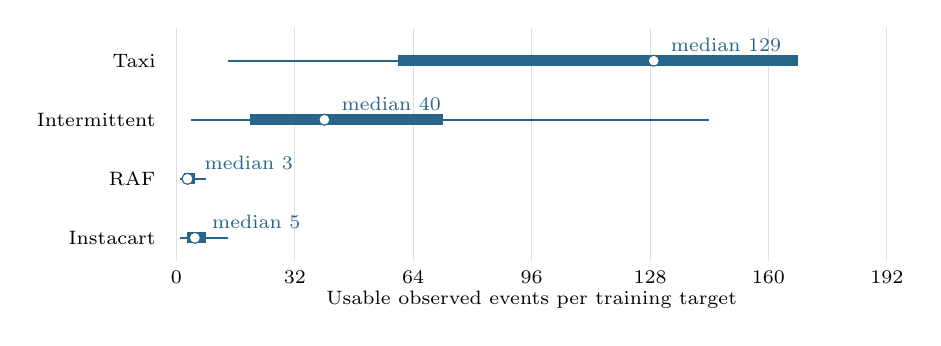
\begin{tikzpicture}[x=.047cm,y=.75cm,font=\scriptsize]
\definecolor{profileblue}{RGB}{40,101,138}
\draw[gray!25] (0,-.4)--(0,3.55);
\node[below] at (0,-.4) {0};
\draw[gray!25] (32,-.4)--(32,3.55);
\node[below] at (32,-.4) {32};
\draw[gray!25] (64,-.4)--(64,3.55);
\node[below] at (64,-.4) {64};
\draw[gray!25] (96,-.4)--(96,3.55);
\node[below] at (96,-.4) {96};
\draw[gray!25] (128,-.4)--(128,3.55);
\node[below] at (128,-.4) {128};
\draw[gray!25] (160,-.4)--(160,3.55);
\node[below] at (160,-.4) {160};
\draw[gray!25] (192,-.4)--(192,3.55);
\node[below] at (192,-.4) {192};
\node[anchor=east] at (-3,3) {Taxi};
\draw[profileblue,line width=.6pt] (14.0,3)--(168.0,3);
\draw[profileblue,line width=4pt] (60.0,3)--(168.0,3);
\filldraw[draw=profileblue,fill=white] (129.0,3) circle[radius=2pt];
\node[anchor=west,text=profileblue] at (131.0,3.27) {median 129};
\node[anchor=east] at (-3,2) {Intermittent};
\draw[profileblue,line width=.6pt] (4.0,2)--(144.0,2);
\draw[profileblue,line width=4pt] (20.0,2)--(72.0,2);
\filldraw[draw=profileblue,fill=white] (40.0,2) circle[radius=2pt];
\node[anchor=west,text=profileblue] at (42.0,2.27) {median 40};
\node[anchor=east] at (-3,1) {RAF};
\draw[profileblue,line width=.6pt] (1.0,1)--(8.0,1);
\draw[profileblue,line width=4pt] (2.0,1)--(5.0,1);
\filldraw[draw=profileblue,fill=white] (3.0,1) circle[radius=2pt];
\node[anchor=west,text=profileblue] at (5.0,1.27) {median 3};
\node[anchor=east] at (-3,0) {Instacart};
\draw[profileblue,line width=.6pt] (1.0,0)--(14.0,0);
\draw[profileblue,line width=4pt] (3.0,0)--(8.0,0);
\filldraw[draw=profileblue,fill=white] (5.0,0) circle[radius=2pt];
\node[anchor=west,text=profileblue] at (7.0,0.27) {median 5};
\node at (96,-1.05) {Usable observed events per training target};
\end{tikzpicture}
\caption{Available training history under the frozen input windows. Thin
lines span the 5th--95th percentiles, thick lines the 25th--75th percentiles,
and circles mark medians. These target-weighted distributions characterize
input availability, not model performance.}
\label{fig:train-history}
\Description{Training-history distributions for four datasets. Taxi and
Intermittent supply longer observed histories than RAF and Instacart.}
\end{figure}

Figure~\ref{fig:train-history} indicates substantial differences in available
history. The median spans 129 observed events on Taxi and 40 on Intermittent,
compared with three on RAF and five on Instacart. Thus an equal nominal
sequence cap would not imply equal evidence per prediction. These training
distributions describe the input populations; they neither measure which
events a trained model retains nor determine its forecasting error.

\section{Event-lag association in the training data}
\label{app:lag}
For series $e$ and event lag $\ell$, pair
$x^{(\ell)}_{e,j}=\log(1+q_{e,j-\ell})$ with
$y^{(\ell)}_{e,j}=\log(1+q_{e,j})$ whenever both events belong to that
training series. Each lag counts observed events in sequence order.
It does not denote elapsed calendar time. The descriptive calculation
includes the complete training sequence, without the model's recorded-time
window or sequence-length cap.

Let $\bar x_e^{(\ell)}$ and $\bar y_e^{(\ell)}$ be the separate means
of the predecessor and successor members of those pairs. The statistic is
\begin{equation}
 r_{\ell}=\operatorname{Corr}\!\left(
 x^{(\ell)}_{e,j}-\bar x_e^{(\ell)},\,
 y^{(\ell)}_{e,j}-\bar y_e^{(\ell)}\right),
 \label{eq:train-lag-correlation}
\end{equation}
where correlation pools the centered pairs across series. Centering removes
between-series differences in mean log quantity, but each pair still
contributes to the pooled sums. This statistic is consequently different
from an average of series-specific correlations. The lag-one column
corresponds to the adjacent log correlation in
Table~\ref{tab:train-characteristics}.
% Generated from reports/titantpp_train_lag_heatmap_20261002_v1/analysis.json.
\begin{figure}[htbp]
\centering
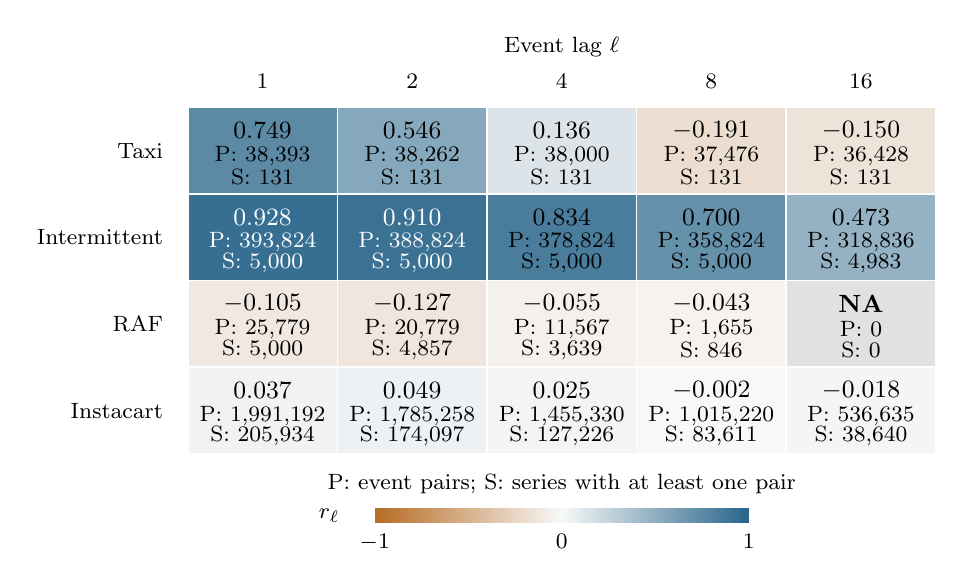
\begin{tikzpicture}[x=1.90cm,y=1.10cm,font=\footnotesize]
\node at (2.5,4.70) {Event lag $\ell$};
\node at (0.5,4.30) {1};
\node at (1.5,4.30) {2};
\node at (2.5,4.30) {4};
\node at (3.5,4.30) {8};
\node at (4.5,4.30) {16};
\node[anchor=east] at (-.10,3.5) {Taxi};
\definecolor{lagcell00}{HTML}{5C8AA5}
\filldraw[fill=lagcell00,draw=white,line width=.6pt] (0,3) rectangle (1,4);
\node[text=black,font=\bfseries\small] at (0.5,3.73) {$0.749$};
\node[text=black,font=\footnotesize] at (0.5,3.44) {P: 38,393};
\node[text=black,font=\footnotesize] at (0.5,3.20) {S: 131};
\definecolor{lagcell01}{HTML}{86A8BC}
\filldraw[fill=lagcell01,draw=white,line width=.6pt] (1,3) rectangle (2,4);
\node[text=black,font=\bfseries\small] at (1.5,3.73) {$0.546$};
\node[text=black,font=\footnotesize] at (1.5,3.44) {P: 38,262};
\node[text=black,font=\footnotesize] at (1.5,3.20) {S: 131};
\definecolor{lagcell02}{HTML}{DCE4E9}
\filldraw[fill=lagcell02,draw=white,line width=.6pt] (2,3) rectangle (3,4);
\node[text=black,font=\bfseries\small] at (2.5,3.73) {$0.136$};
\node[text=black,font=\footnotesize] at (2.5,3.44) {P: 38,000};
\node[text=black,font=\footnotesize] at (2.5,3.20) {S: 131};
\definecolor{lagcell03}{HTML}{EBDDCF}
\filldraw[fill=lagcell03,draw=white,line width=.6pt] (3,3) rectangle (4,4);
\node[text=black,font=\bfseries\small] at (3.5,3.73) {$-0.191$};
\node[text=black,font=\footnotesize] at (3.5,3.44) {P: 37,476};
\node[text=black,font=\footnotesize] at (3.5,3.20) {S: 131};
\definecolor{lagcell04}{HTML}{EEE3D8}
\filldraw[fill=lagcell04,draw=white,line width=.6pt] (4,3) rectangle (5,4);
\node[text=black,font=\bfseries\small] at (4.5,3.73) {$-0.150$};
\node[text=black,font=\footnotesize] at (4.5,3.44) {P: 36,428};
\node[text=black,font=\footnotesize] at (4.5,3.20) {S: 131};
\node[anchor=east] at (-.10,2.5) {Intermittent};
\definecolor{lagcell10}{HTML}{376F92}
\filldraw[fill=lagcell10,draw=white,line width=.6pt] (0,2) rectangle (1,3);
\node[text=white,font=\bfseries\small] at (0.5,2.73) {$0.928$};
\node[text=white,font=\footnotesize] at (0.5,2.44) {P: 393,824};
\node[text=white,font=\footnotesize] at (0.5,2.20) {S: 5,000};
\definecolor{lagcell11}{HTML}{3B7294}
\filldraw[fill=lagcell11,draw=white,line width=.6pt] (1,2) rectangle (2,3);
\node[text=white,font=\bfseries\small] at (1.5,2.73) {$0.910$};
\node[text=white,font=\footnotesize] at (1.5,2.44) {P: 388,824};
\node[text=white,font=\footnotesize] at (1.5,2.20) {S: 5,000};
\definecolor{lagcell12}{HTML}{4A7D9C}
\filldraw[fill=lagcell12,draw=white,line width=.6pt] (2,2) rectangle (3,3);
\node[text=black,font=\bfseries\small] at (2.5,2.73) {$0.834$};
\node[text=black,font=\footnotesize] at (2.5,2.44) {P: 378,824};
\node[text=black,font=\footnotesize] at (2.5,2.20) {S: 5,000};
\definecolor{lagcell13}{HTML}{6691AB}
\filldraw[fill=lagcell13,draw=white,line width=.6pt] (3,2) rectangle (4,3);
\node[text=black,font=\bfseries\small] at (3.5,2.73) {$0.700$};
\node[text=black,font=\footnotesize] at (3.5,2.44) {P: 358,824};
\node[text=black,font=\footnotesize] at (3.5,2.20) {S: 5,000};
\definecolor{lagcell14}{HTML}{95B2C4}
\filldraw[fill=lagcell14,draw=white,line width=.6pt] (4,2) rectangle (5,3);
\node[text=black,font=\bfseries\small] at (4.5,2.73) {$0.473$};
\node[text=black,font=\footnotesize] at (4.5,2.44) {P: 318,836};
\node[text=black,font=\footnotesize] at (4.5,2.20) {S: 4,983};
\node[anchor=east] at (-.10,1.5) {RAF};
\definecolor{lagcell20}{HTML}{F1E9E1}
\filldraw[fill=lagcell20,draw=white,line width=.6pt] (0,1) rectangle (1,2);
\node[text=black,font=\bfseries\small] at (0.5,1.73) {$-0.105$};
\node[text=black,font=\footnotesize] at (0.5,1.44) {P: 25,779};
\node[text=black,font=\footnotesize] at (0.5,1.20) {S: 5,000};
\definecolor{lagcell21}{HTML}{F0E6DD}
\filldraw[fill=lagcell21,draw=white,line width=.6pt] (1,1) rectangle (2,2);
\node[text=black,font=\bfseries\small] at (1.5,1.73) {$-0.127$};
\node[text=black,font=\footnotesize] at (1.5,1.44) {P: 20,779};
\node[text=black,font=\footnotesize] at (1.5,1.20) {S: 4,857};
\definecolor{lagcell22}{HTML}{F4F0EC}
\filldraw[fill=lagcell22,draw=white,line width=.6pt] (2,1) rectangle (3,2);
\node[text=black,font=\bfseries\small] at (2.5,1.73) {$-0.055$};
\node[text=black,font=\footnotesize] at (2.5,1.44) {P: 11,567};
\node[text=black,font=\footnotesize] at (2.5,1.20) {S: 3,639};
\definecolor{lagcell23}{HTML}{F5F2EF}
\filldraw[fill=lagcell23,draw=white,line width=.6pt] (3,1) rectangle (4,2);
\node[text=black,font=\bfseries\small] at (3.5,1.73) {$-0.043$};
\node[text=black,font=\footnotesize] at (3.5,1.44) {P: 1,655};
\node[text=black,font=\footnotesize] at (3.5,1.20) {S: 846};
\definecolor{lagcell24}{HTML}{E1E1E1}
\filldraw[fill=lagcell24,draw=white,line width=.6pt] (4,1) rectangle (5,2);
\node[text=black,font=\bfseries\small] at (4.5,1.73) {NA};
\node[text=black,font=\footnotesize] at (4.5,1.44) {P: 0};
\node[text=black,font=\footnotesize] at (4.5,1.20) {S: 0};
\node[anchor=east] at (-.10,0.5) {Instacart};
\definecolor{lagcell30}{HTML}{F0F2F4}
\filldraw[fill=lagcell30,draw=white,line width=.6pt] (0,0) rectangle (1,1);
\node[text=black,font=\bfseries\small] at (0.5,0.73) {$0.037$};
\node[text=black,font=\footnotesize] at (0.5,0.44) {P: 1,991,192};
\node[text=black,font=\footnotesize] at (0.5,0.20) {S: 205,934};
\definecolor{lagcell31}{HTML}{EEF1F3}
\filldraw[fill=lagcell31,draw=white,line width=.6pt] (1,0) rectangle (2,1);
\node[text=black,font=\bfseries\small] at (1.5,0.73) {$0.049$};
\node[text=black,font=\footnotesize] at (1.5,0.44) {P: 1,785,258};
\node[text=black,font=\footnotesize] at (1.5,0.20) {S: 174,097};
\definecolor{lagcell32}{HTML}{F3F4F5}
\filldraw[fill=lagcell32,draw=white,line width=.6pt] (2,0) rectangle (3,1);
\node[text=black,font=\bfseries\small] at (2.5,0.73) {$0.025$};
\node[text=black,font=\footnotesize] at (2.5,0.44) {P: 1,455,330};
\node[text=black,font=\footnotesize] at (2.5,0.20) {S: 127,226};
\definecolor{lagcell33}{HTML}{F8F8F8}
\filldraw[fill=lagcell33,draw=white,line width=.6pt] (3,0) rectangle (4,1);
\node[text=black,font=\bfseries\small] at (3.5,0.73) {$-0.002$};
\node[text=black,font=\footnotesize] at (3.5,0.44) {P: 1,015,220};
\node[text=black,font=\footnotesize] at (3.5,0.20) {S: 83,611};
\definecolor{lagcell34}{HTML}{F7F5F4}
\filldraw[fill=lagcell34,draw=white,line width=.6pt] (4,0) rectangle (5,1);
\node[text=black,font=\bfseries\small] at (4.5,0.73) {$-0.018$};
\node[text=black,font=\footnotesize] at (4.5,0.44) {P: 536,635};
\node[text=black,font=\footnotesize] at (4.5,0.20) {S: 38,640};
\node at (2.5,-.35) {P: event pairs; S: series with at least one pair};
\definecolor{lagbar0}{HTML}{B76C25}
\fill[lagbar0] (1.2500,-.80) rectangle (1.2750,-.62);
\definecolor{lagbar1}{HTML}{B86F29}
\fill[lagbar1] (1.2750,-.80) rectangle (1.3000,-.62);
\definecolor{lagbar2}{HTML}{B9722E}
\fill[lagbar2] (1.3000,-.80) rectangle (1.3250,-.62);
\definecolor{lagbar3}{HTML}{BB7532}
\fill[lagbar3] (1.3250,-.80) rectangle (1.3500,-.62);
\definecolor{lagbar4}{HTML}{BC7836}
\fill[lagbar4] (1.3500,-.80) rectangle (1.3750,-.62);
\definecolor{lagbar5}{HTML}{BD7B3A}
\fill[lagbar5] (1.3750,-.80) rectangle (1.4000,-.62);
\definecolor{lagbar6}{HTML}{BF7D3F}
\fill[lagbar6] (1.4000,-.80) rectangle (1.4250,-.62);
\definecolor{lagbar7}{HTML}{C08043}
\fill[lagbar7] (1.4250,-.80) rectangle (1.4500,-.62);
\definecolor{lagbar8}{HTML}{C18347}
\fill[lagbar8] (1.4500,-.80) rectangle (1.4750,-.62);
\definecolor{lagbar9}{HTML}{C3864B}
\fill[lagbar9] (1.4750,-.80) rectangle (1.5000,-.62);
\definecolor{lagbar10}{HTML}{C48950}
\fill[lagbar10] (1.5000,-.80) rectangle (1.5250,-.62);
\definecolor{lagbar11}{HTML}{C58B54}
\fill[lagbar11] (1.5250,-.80) rectangle (1.5500,-.62);
\definecolor{lagbar12}{HTML}{C68E58}
\fill[lagbar12] (1.5500,-.80) rectangle (1.5750,-.62);
\definecolor{lagbar13}{HTML}{C8915D}
\fill[lagbar13] (1.5750,-.80) rectangle (1.6000,-.62);
\definecolor{lagbar14}{HTML}{C99461}
\fill[lagbar14] (1.6000,-.80) rectangle (1.6250,-.62);
\definecolor{lagbar15}{HTML}{CA9765}
\fill[lagbar15] (1.6250,-.80) rectangle (1.6500,-.62);
\definecolor{lagbar16}{HTML}{CC9A69}
\fill[lagbar16] (1.6500,-.80) rectangle (1.6750,-.62);
\definecolor{lagbar17}{HTML}{CD9C6E}
\fill[lagbar17] (1.6750,-.80) rectangle (1.7000,-.62);
\definecolor{lagbar18}{HTML}{CE9F72}
\fill[lagbar18] (1.7000,-.80) rectangle (1.7250,-.62);
\definecolor{lagbar19}{HTML}{D0A276}
\fill[lagbar19] (1.7250,-.80) rectangle (1.7500,-.62);
\definecolor{lagbar20}{HTML}{D1A57A}
\fill[lagbar20] (1.7500,-.80) rectangle (1.7750,-.62);
\definecolor{lagbar21}{HTML}{D2A87F}
\fill[lagbar21] (1.7750,-.80) rectangle (1.8000,-.62);
\definecolor{lagbar22}{HTML}{D4AA83}
\fill[lagbar22] (1.8000,-.80) rectangle (1.8250,-.62);
\definecolor{lagbar23}{HTML}{D5AD87}
\fill[lagbar23] (1.8250,-.80) rectangle (1.8500,-.62);
\definecolor{lagbar24}{HTML}{D6B08B}
\fill[lagbar24] (1.8500,-.80) rectangle (1.8750,-.62);
\definecolor{lagbar25}{HTML}{D8B390}
\fill[lagbar25] (1.8750,-.80) rectangle (1.9000,-.62);
\definecolor{lagbar26}{HTML}{D9B694}
\fill[lagbar26] (1.9000,-.80) rectangle (1.9250,-.62);
\definecolor{lagbar27}{HTML}{DAB998}
\fill[lagbar27] (1.9250,-.80) rectangle (1.9500,-.62);
\definecolor{lagbar28}{HTML}{DCBB9C}
\fill[lagbar28] (1.9500,-.80) rectangle (1.9750,-.62);
\definecolor{lagbar29}{HTML}{DDBEA1}
\fill[lagbar29] (1.9750,-.80) rectangle (2.0000,-.62);
\definecolor{lagbar30}{HTML}{DEC1A5}
\fill[lagbar30] (2.0000,-.80) rectangle (2.0250,-.62);
\definecolor{lagbar31}{HTML}{E0C4A9}
\fill[lagbar31] (2.0250,-.80) rectangle (2.0500,-.62);
\definecolor{lagbar32}{HTML}{E1C7AD}
\fill[lagbar32] (2.0500,-.80) rectangle (2.0750,-.62);
\definecolor{lagbar33}{HTML}{E2C9B2}
\fill[lagbar33] (2.0750,-.80) rectangle (2.1000,-.62);
\definecolor{lagbar34}{HTML}{E4CCB6}
\fill[lagbar34] (2.1000,-.80) rectangle (2.1250,-.62);
\definecolor{lagbar35}{HTML}{E5CFBA}
\fill[lagbar35] (2.1250,-.80) rectangle (2.1500,-.62);
\definecolor{lagbar36}{HTML}{E6D2BE}
\fill[lagbar36] (2.1500,-.80) rectangle (2.1750,-.62);
\definecolor{lagbar37}{HTML}{E8D5C3}
\fill[lagbar37] (2.1750,-.80) rectangle (2.2000,-.62);
\definecolor{lagbar38}{HTML}{E9D8C7}
\fill[lagbar38] (2.2000,-.80) rectangle (2.2250,-.62);
\definecolor{lagbar39}{HTML}{EADACB}
\fill[lagbar39] (2.2250,-.80) rectangle (2.2500,-.62);
\definecolor{lagbar40}{HTML}{EBDDD0}
\fill[lagbar40] (2.2500,-.80) rectangle (2.2750,-.62);
\definecolor{lagbar41}{HTML}{EDE0D4}
\fill[lagbar41] (2.2750,-.80) rectangle (2.3000,-.62);
\definecolor{lagbar42}{HTML}{EEE3D8}
\fill[lagbar42] (2.3000,-.80) rectangle (2.3250,-.62);
\definecolor{lagbar43}{HTML}{EFE6DC}
\fill[lagbar43] (2.3250,-.80) rectangle (2.3500,-.62);
\definecolor{lagbar44}{HTML}{F1E8E1}
\fill[lagbar44] (2.3500,-.80) rectangle (2.3750,-.62);
\definecolor{lagbar45}{HTML}{F2EBE5}
\fill[lagbar45] (2.3750,-.80) rectangle (2.4000,-.62);
\definecolor{lagbar46}{HTML}{F3EEE9}
\fill[lagbar46] (2.4000,-.80) rectangle (2.4250,-.62);
\definecolor{lagbar47}{HTML}{F5F1ED}
\fill[lagbar47] (2.4250,-.80) rectangle (2.4500,-.62);
\definecolor{lagbar48}{HTML}{F6F4F2}
\fill[lagbar48] (2.4500,-.80) rectangle (2.4750,-.62);
\definecolor{lagbar49}{HTML}{F7F7F6}
\fill[lagbar49] (2.4750,-.80) rectangle (2.5000,-.62);
\definecolor{lagbar50}{HTML}{F6F7F7}
\fill[lagbar50] (2.5000,-.80) rectangle (2.5250,-.62);
\definecolor{lagbar51}{HTML}{F2F4F5}
\fill[lagbar51] (2.5250,-.80) rectangle (2.5500,-.62);
\definecolor{lagbar52}{HTML}{EEF1F2}
\fill[lagbar52] (2.5500,-.80) rectangle (2.5750,-.62);
\definecolor{lagbar53}{HTML}{E9EEF0}
\fill[lagbar53] (2.5750,-.80) rectangle (2.6000,-.62);
\definecolor{lagbar54}{HTML}{E5EBEE}
\fill[lagbar54] (2.6000,-.80) rectangle (2.6250,-.62);
\definecolor{lagbar55}{HTML}{E1E8EC}
\fill[lagbar55] (2.6250,-.80) rectangle (2.6500,-.62);
\definecolor{lagbar56}{HTML}{DDE5EA}
\fill[lagbar56] (2.6500,-.80) rectangle (2.6750,-.62);
\definecolor{lagbar57}{HTML}{D9E2E7}
\fill[lagbar57] (2.6750,-.80) rectangle (2.7000,-.62);
\definecolor{lagbar58}{HTML}{D5DFE5}
\fill[lagbar58] (2.7000,-.80) rectangle (2.7250,-.62);
\definecolor{lagbar59}{HTML}{D0DCE3}
\fill[lagbar59] (2.7250,-.80) rectangle (2.7500,-.62);
\definecolor{lagbar60}{HTML}{CCD9E1}
\fill[lagbar60] (2.7500,-.80) rectangle (2.7750,-.62);
\definecolor{lagbar61}{HTML}{C8D6DF}
\fill[lagbar61] (2.7750,-.80) rectangle (2.8000,-.62);
\definecolor{lagbar62}{HTML}{C4D3DC}
\fill[lagbar62] (2.8000,-.80) rectangle (2.8250,-.62);
\definecolor{lagbar63}{HTML}{C0D0DA}
\fill[lagbar63] (2.8250,-.80) rectangle (2.8500,-.62);
\definecolor{lagbar64}{HTML}{BCCDD8}
\fill[lagbar64] (2.8500,-.80) rectangle (2.8750,-.62);
\definecolor{lagbar65}{HTML}{B8CAD6}
\fill[lagbar65] (2.8750,-.80) rectangle (2.9000,-.62);
\definecolor{lagbar66}{HTML}{B3C7D4}
\fill[lagbar66] (2.9000,-.80) rectangle (2.9250,-.62);
\definecolor{lagbar67}{HTML}{AFC5D2}
\fill[lagbar67] (2.9250,-.80) rectangle (2.9500,-.62);
\definecolor{lagbar68}{HTML}{ABC2CF}
\fill[lagbar68] (2.9500,-.80) rectangle (2.9750,-.62);
\definecolor{lagbar69}{HTML}{A7BFCD}
\fill[lagbar69] (2.9750,-.80) rectangle (3.0000,-.62);
\definecolor{lagbar70}{HTML}{A3BCCB}
\fill[lagbar70] (3.0000,-.80) rectangle (3.0250,-.62);
\definecolor{lagbar71}{HTML}{9FB9C9}
\fill[lagbar71] (3.0250,-.80) rectangle (3.0500,-.62);
\definecolor{lagbar72}{HTML}{9AB6C6}
\fill[lagbar72] (3.0500,-.80) rectangle (3.0750,-.62);
\definecolor{lagbar73}{HTML}{96B3C4}
\fill[lagbar73] (3.0750,-.80) rectangle (3.1000,-.62);
\definecolor{lagbar74}{HTML}{92B0C2}
\fill[lagbar74] (3.1000,-.80) rectangle (3.1250,-.62);
\definecolor{lagbar75}{HTML}{8EADC0}
\fill[lagbar75] (3.1250,-.80) rectangle (3.1500,-.62);
\definecolor{lagbar76}{HTML}{8AAABE}
\fill[lagbar76] (3.1500,-.80) rectangle (3.1750,-.62);
\definecolor{lagbar77}{HTML}{86A7BB}
\fill[lagbar77] (3.1750,-.80) rectangle (3.2000,-.62);
\definecolor{lagbar78}{HTML}{81A4B9}
\fill[lagbar78] (3.2000,-.80) rectangle (3.2250,-.62);
\definecolor{lagbar79}{HTML}{7DA1B7}
\fill[lagbar79] (3.2250,-.80) rectangle (3.2500,-.62);
\definecolor{lagbar80}{HTML}{799EB5}
\fill[lagbar80] (3.2500,-.80) rectangle (3.2750,-.62);
\definecolor{lagbar81}{HTML}{759BB3}
\fill[lagbar81] (3.2750,-.80) rectangle (3.3000,-.62);
\definecolor{lagbar82}{HTML}{7198B0}
\fill[lagbar82] (3.3000,-.80) rectangle (3.3250,-.62);
\definecolor{lagbar83}{HTML}{6D96AE}
\fill[lagbar83] (3.3250,-.80) rectangle (3.3500,-.62);
\definecolor{lagbar84}{HTML}{6893AC}
\fill[lagbar84] (3.3500,-.80) rectangle (3.3750,-.62);
\definecolor{lagbar85}{HTML}{6490AA}
\fill[lagbar85] (3.3750,-.80) rectangle (3.4000,-.62);
\definecolor{lagbar86}{HTML}{608DA8}
\fill[lagbar86] (3.4000,-.80) rectangle (3.4250,-.62);
\definecolor{lagbar87}{HTML}{5C8AA5}
\fill[lagbar87] (3.4250,-.80) rectangle (3.4500,-.62);
\definecolor{lagbar88}{HTML}{5887A3}
\fill[lagbar88] (3.4500,-.80) rectangle (3.4750,-.62);
\definecolor{lagbar89}{HTML}{5484A1}
\fill[lagbar89] (3.4750,-.80) rectangle (3.5000,-.62);
\definecolor{lagbar90}{HTML}{50819F}
\fill[lagbar90] (3.5000,-.80) rectangle (3.5250,-.62);
\definecolor{lagbar91}{HTML}{4B7E9D}
\fill[lagbar91] (3.5250,-.80) rectangle (3.5500,-.62);
\definecolor{lagbar92}{HTML}{477B9A}
\fill[lagbar92] (3.5500,-.80) rectangle (3.5750,-.62);
\definecolor{lagbar93}{HTML}{437898}
\fill[lagbar93] (3.5750,-.80) rectangle (3.6000,-.62);
\definecolor{lagbar94}{HTML}{3F7596}
\fill[lagbar94] (3.6000,-.80) rectangle (3.6250,-.62);
\definecolor{lagbar95}{HTML}{3B7294}
\fill[lagbar95] (3.6250,-.80) rectangle (3.6500,-.62);
\definecolor{lagbar96}{HTML}{376F92}
\fill[lagbar96] (3.6500,-.80) rectangle (3.6750,-.62);
\definecolor{lagbar97}{HTML}{326C90}
\fill[lagbar97] (3.6750,-.80) rectangle (3.7000,-.62);
\definecolor{lagbar98}{HTML}{2E698D}
\fill[lagbar98] (3.7000,-.80) rectangle (3.7250,-.62);
\definecolor{lagbar99}{HTML}{2A668B}
\fill[lagbar99] (3.7250,-.80) rectangle (3.7500,-.62);
\node[below] at (1.25,-.81) {$-1$};
\node[below] at (2.5,-.81) {$0$};
\node[below] at (3.75,-.81) {$1$};
\node[anchor=east] at (1.08,-.71) {$r_{\ell}$};
\end{tikzpicture}
\caption{Train-only within-series log-quantity correlation at event lags 1, 2, 4, 8, and 16. Each cell reports $r_{\ell}$, the number of event pairs (P), and the number of contributing series (S). All cells share the color scale $[-1,1]$; gray NA denotes no available pairs. Pair counts include constant and single-pair series, which contribute zero to one or both centered sums of squares. Pairs cover complete training sequences without input-window or sequence-cap restrictions.}
\label{fig:train-lag-correlation}
\Description{A four-by-five heatmap. Taxi correlation declines from 0.749 at lag one to negative values at lags eight and sixteen. Intermittent remains positive, declining from 0.928 to 0.473. RAF has small negative correlations through lag eight and no pairs at lag sixteen. Instacart correlations remain close to zero. Pair and series counts are printed in every cell.}
\end{figure}

Taxi's association declines with event lag, while Intermittent retains
positive association over the displayed range. RAF supplies comparatively
few long-lag pairs, and Instacart's correlations remain close to zero.
Counts in Figure~\ref{fig:train-lag-correlation} matter because the available
series and pairs change with lag. A series with one pair contributes zero
to both centered sums of squares. Constant pairs also provide no variation,
and a zero pooled denominator leaves the correlation undefined.
RAF's negative values therefore describe these centered samples without
establishing a general law of negative dependence.

An archived sensitivity calculation restricts every lag to the same series
with at least 20 training events. This cohort retains 131 Taxi series,
4,968 Intermittent series, and 31,020 Instacart series; RAF supplies none.
Instacart's lag-one and lag-two correlations increase to 0.074 and 0.092
in this cohort. The change cautions against treating the full-population
profile as invariant to series composition.

Event-lag association provides a descriptive motivation for examining local
and recurrent history paths. It does not measure the contribution of either
path. CNN+GRU54 processes contextual states within the retained input window,
whereas Eq.~\eqref{eq:train-lag-correlation} describes unconditional
log-quantity pairs across complete training sequences. Neither the sign nor
the magnitude of $r_{\ell}$ establishes a correction gain, a preferred
recurrent width, or an architectural ranking. Those claims depend on the
matched validation comparisons specified in the main text.

\section{Diagnostic partitions and aggregation}
\label{app:strata}
\subsection{Quantity and usable-history partitions}
Stratification distinguishes a change in errors within a group from a change
in that group's contribution to the aggregate. The quantity boundaries are
the training-derived 50th, 90th, 95th, and 99th percentiles, namely
$(7,686,1562,3449)$ for Taxi, $(2,31,46,187)$ for Intermittent,
$(2,30,60,200)$ for RAF, and $(8,20,25,35)$ for Instacart.
Each upper boundary belongs to the lower bin, so the last bin agrees with
the strict large-quantity threshold in Table~\ref{tab:data}.

The stored history partitions divide Taxi, Intermittent, and RAF at 64 and
128 usable events, and Instacart at 1, 3, 7, 15, and 31. They permit
within-dataset diagnosis, although they do not define identical groups
across datasets. Their resolution also depends on the sequence cap.
Empty strata remain explicit and receive no estimated error. For a fixed
dataset, every comparison arm and seed must share target membership and
partition boundaries.

All strata inherit the checkpoint selected by minimum overall validation
quantity RMSE. Neither a favorable bin nor a timing score changes that
selection. A prespecified control remains fixed across bins; if an external
comparator is selected by aggregate validation RMSE, that same comparator
also remains fixed. These rules prevent a separate best-model choice within
each subgroup. The definitions below specify the diagnostic procedure and
introduce no additional CNN+GRU performance results.

\subsection{Per-seed errors and additive contributions}
For model $m$, seed $s$, and a nonempty stratum $b$ containing $N_b$
targets, define
\begin{align}
 \mathrm{SSE}_{m,s,b}&=\sum_{i\in b}(\widehat q_{m,s,i}-q_i)^2,\\
 \mathrm{MAE}_{m,s,b}&=\frac{1}{N_b}\sum_{i\in b}
       |\widehat q_{m,s,i}-q_i|,\qquad
 \mathrm{RMSE}_{m,s,b}=\sqrt{\frac{\mathrm{SSE}_{m,s,b}}{N_b}}.
 \label{eq:stratum-errors}
\end{align}
Compute each metric within a seed before averaging over
$\mathcal S=\{42,52,62\}$. Sample standard deviations describe the dispersion
of these seed-level metrics. The count $N_b$ refers to targets in one seed,
rather than repeated copies of the same target across seeds.

Let $M$ denote the focal model, $C$ its fixed comparator, and
$N=\sum_bN_b$. The contributions of bin $b$ to the aggregate differences are
\begin{align}
 C_b^{\rm MSE}&=\frac{1}{|\mathcal S|N}\sum_{s\in\mathcal S}
  (\mathrm{SSE}_{M,s,b}-\mathrm{SSE}_{C,s,b}),
  \label{eq:strata-mse-contribution}\\
 C_b^{\rm MAE}&=\frac{N_b}{N|\mathcal S|}\sum_{s\in\mathcal S}
  (\mathrm{MAE}_{M,s,b}-\mathrm{MAE}_{C,s,b}).
  \label{eq:strata-mae-contribution}
\end{align}
Summing these contributions across bins recovers the mean of the seeds'
overall MSE or MAE differences. Negative values favor $M$. The MSE sum is
not the difference between squared mean RMSEs, and binwise RMSE differences
do not supply an additive decomposition. Empty bins contribute zero to the
aggregate through their zero target count, without an estimated bin metric.

Because each contribution includes target share, a small group with large
errors can offset gains across a larger group. Reporting both within-bin
errors and contributions distinguishes these cases without attributing the
difference to a single data characteristic. A model-specific decomposition
requires that model's selected-checkpoint validation records. Historical
MLP decompositions cannot substitute for CNN+GRU54 results.

\end{document}
